\documentclass[11pt,a4paper]{article}

% ---------- Page layout and fonts ----------
\usepackage[a4paper,top=2.5cm,bottom=2.5cm,left=2.5cm,right=2.5cm,headheight=14pt]{geometry}
\usepackage{newtxtext,newtxmath}
\usepackage{fontspec}
\setmonofont{Inconsolatazi4-Regular.otf}[Scale=0.88, BoldFont=Inconsolatazi4-Bold.otf]
\usepackage{microtype}
\usepackage{setspace}
\setstretch{1.08}
\usepackage[parfill]{parskip}

% ---------- Tables, figures, captions ----------
\usepackage{booktabs,tabularx,multirow,array,longtable}
\usepackage{graphicx}
\usepackage{float}
\usepackage[font=small,labelfont=bf,margin=0.5cm]{caption}
\usepackage{subcaption}
\usepackage{xcolor}
\usepackage{enumitem}
\setlist{itemsep=2pt,topsep=4pt}
\usepackage{siunitx}
\sisetup{group-separator={,},group-minimum-digits=4}

% ---------- Charts and diagrams ----------
\usepackage{pgfplots}
\pgfplotsset{compat=1.18}
\usepgfplotslibrary{groupplots}
\usetikzlibrary{arrows.meta,positioning,shapes.geometric,fit,calc,patterns,backgrounds}

\definecolor{cprev}{HTML}{B03A2E}   % previous / before
\definecolor{cnew}{HTML}{1F6F8B}    % new / after
\definecolor{cthird}{HTML}{6C8E3B}
\definecolor{cfourth}{HTML}{C9892B}
\definecolor{cgrey}{HTML}{8A8F98}
\definecolor{boxblue}{HTML}{E8F1F6}
\definecolor{boxgreen}{HTML}{EAF3E3}
\definecolor{boxamber}{HTML}{FBF1E1}
\definecolor{boxgrey}{HTML}{F2F3F5}
\definecolor{linkblue}{HTML}{1A3D7C}

\pgfplotsset{
  reportbars/.style={
    ybar, axis lines*=left, ymajorgrids, grid style={dashed,gray!35},
    tick label style={font=\footnotesize}, label style={font=\small},
    legend style={font=\footnotesize, draw=none, fill=none, legend columns=-1, at={(0.5,-0.18)}, anchor=north},
    nodes near coords style={font=\scriptsize},
    enlarge x limits=0.08,
    legend image code/.code={\draw[#1, draw=none] (0cm,-0.08cm) rectangle (0.32cm,0.14cm);},
  },
}

% ---------- Header / footer ----------
\usepackage{fancyhdr}
\pagestyle{fancy}
\fancyhf{}
\fancyhead[L]{\small\textbf{Optimizing a CI/CD Localization Pipeline on AWS}}
\fancyhead[R]{\small BITS Pilani, Hyderabad Campus}
\fancyfoot[C]{\small\thepage}
\renewcommand{\headrulewidth}{0.4pt}

% ---------- Section style ----------
\usepackage{titlesec}
\titleformat{\section}{\Large\bfseries}{\thesection}{0.8em}{}
\titleformat{\subsection}{\large\bfseries}{\thesubsection}{0.7em}{}
\titleformat{\subsubsection}{\normalsize\bfseries}{\thesubsubsection}{0.6em}{}
\titlespacing*{\section}{0pt}{16pt}{8pt}
\titlespacing*{\subsection}{0pt}{12pt}{5pt}

% ---------- Links ----------
\usepackage[hidelinks]{hyperref}
\hypersetup{colorlinks=true,linkcolor=linkblue,urlcolor=linkblue,citecolor=linkblue}
\usepackage{bookmark}

% ---------- Small helpers ----------
\newcommand{\code}[1]{\texttt{#1}}
\newcommand{\x}{$\times$}
\newcolumntype{L}{>{\raggedright\arraybackslash}X}
\newcolumntype{R}{>{\raggedleft\arraybackslash}X}
\newcommand{\keyresult}[1]{%
  \par\smallskip\noindent\fcolorbox{cnew!60}{boxblue}{\parbox{\dimexpr\linewidth-2\fboxsep-2\fboxrule\relax}{\small #1}}\par\smallskip}

% ---------- Team ----------
\newcommand{\reporttitle}{Optimizing a CI/CD Software Localization Pipeline on AWS}
\newcommand{\reportsubtitle}{Token-Efficient Batching and a Persistent Translation Memory}

\begin{document}

% =================== Title page ===================
\begin{titlepage}
\thispagestyle{empty}
\centering
\vspace*{0.2cm}

\includegraphics[width=2.4cm]{figures/bits_logo.png}\par\vspace{0.6cm}
{\LARGE\bfseries BIRLA INSTITUTE OF TECHNOLOGY AND\\SCIENCE, PILANI\par}
\vspace{0.25cm}
{\large Hyderabad Campus\par}
{\large Department of Computer Science and Information Systems\par}
\vspace{0.8cm}
{\huge\bfseries End-Semester Project Report\par}
\vspace{0.7cm}
{\Large\bfseries \reporttitle\par}
\vspace{0.3cm}
{\large\itshape \reportsubtitle\par}
\vspace{0.8cm}
\rule{0.55\linewidth}{0.4pt}\par\vspace{0.3cm}
Submitted as part of the requirements for\par
{\large\bfseries Research Practice\par}
\vspace{0.15cm}
Under the supervision of\par
{\large\bfseries Prof.\ Subhrakanta Panda\par}
\vspace{0.3cm}
\rule{0.55\linewidth}{0.4pt}\par
\vspace{0.7cm}
{\large\bfseries Submitted by\par}
\vspace{0.3cm}
\begin{tabular}{|l|l|}
\hline
\textbf{Name} & \textbf{ID} \\ \hline
Tanish Kumar Gupta & 2025H1030061H \\
Aayush Gupt & 2025H1030042H \\
Alok Singh & 2025H1030067H \\
Akshad Ajay Kalaskar & 2025H1030065H \\ \hline
\end{tabular}
\par\vfill
{\large End-Semester Submission \,$\cdot$\, Academic Year 2026--2027\par}
\end{titlepage}

\pagenumbering{roman}

% =================== Certificate ===================
\section*{Certificate}
\addcontentsline{toc}{section}{Certificate}
This is to certify that the project titled \textbf{\reporttitle: \reportsubtitle} has been carried out by
\mbox{\textbf{Tanish Kumar Gupta}}, \mbox{\textbf{Aayush Gupt}}, \mbox{\textbf{Alok Singh}} and \mbox{\textbf{Akshad Ajay Kalaskar}} under my supervision as part of the
Research Practice requirement at BITS Pilani, Hyderabad Campus.

The work presented in this report continues the previous semester's localization pipeline. It moves the pipeline to
Amazon Web Services, profiles its translation stage, redesigns its batching logic for token efficiency, adds safeguards
for software placeholders and untranslatable characters, and rebuilds its Translation Memory so that continuous-integration
runs translate only what has changed. Every result is backed by recorded runs on the KDE4 software-localization corpus in
twelve languages.

\vspace{2.5cm}
\hfill\begin{tabular}{c}
\rule{6.5cm}{0.4pt}\\
\textbf{Prof.\ Subhrakanta Panda}\\
Department of Computer Science and\\
Information Systems\\
BITS Pilani, Hyderabad Campus
\end{tabular}
\clearpage

% =================== Acknowledgement ===================
\section*{Acknowledgement}
\addcontentsline{toc}{section}{Acknowledgement}
We thank \textbf{Prof.\ Subhrakanta Panda} for his guidance throughout the semester. His insistence on measuring every
change, and on separating what was measured from what was estimated, shaped the experimental method used in this report.

We thank the \textbf{Department of Computer Science and Information Systems}, BITS Pilani, Hyderabad Campus, for the
academic environment and resources that made this work possible, and the Track~1 team for preparing and cleaning the
twelve-language KDE4 dataset used throughout our evaluation.

We also acknowledge the open-source communities behind \textbf{NLLB-200}, \textbf{CTranslate2}, \textbf{Hugging Face
Transformers}, \textbf{SacreBLEU}, the \textbf{OPUS KDE4} corpus and the \textbf{FLORES-200} benchmark.
\clearpage

% =================== Abstract ===================
\section*{Abstract}
\addcontentsline{toc}{section}{Abstract}
This report documents the second semester of work on an automated software-localization pipeline that translates
\code{.resx} resource files into multiple languages inside a continuous-integration (CI/CD) workflow. The pipeline was
moved from Microsoft Azure to Amazon Web Services (AWS) with its translation logic unchanged, and then optimized in three
steps, each measured on the KDE4 software-localization corpus in twelve languages.

\textbf{Batching.} Profiling showed that model inference takes 99.3\% of the translation stage, that mixed-length batches
wasted 30\% of the model's input on padding, and that the machine's two cores were only 59\% busy. Sorting strings by
length cut padding to 4\% but gained only 3\%: padding was not the bottleneck. Reducing the beam size from 5 to 2 made
translation 2.2\x{} faster for a 0.45-point chrF loss, and translating two batches in parallel with an output length cap
added 1.27\x{} with identical output. A full production run translated all 10,054 usable KDE4 strings into 12 languages
(120,648 translations) in 3.6 hours with no failures, about 2.5\x{} faster than the semester's starting configuration.

\textbf{Quality safeguards.} Placeholder protection raised the share of strings whose placeholders survive translation
from 87.7\% to 99.88\%. The run also revealed that 6.1\% of Chinese outputs silently lost characters the model cannot
write; these strings are now kept in English and reported instead of being shipped broken.

\textbf{Translation Memory.} The memory was rebuilt to persist between runs, to record which model and settings produced
each translation, to load once per language per run, and to reuse near-identical strings. In a simulated CI/CD history,
commits that change 1\%, 5\% and 10\% of an application ran 25\x{}, 14\x{} and 8.4\x{} faster than the previous
pipeline with 98.4\%, 95.0\% and 90.6\% fewer model tokens, at unchanged quality (chrF 63.38 versus 63.37). Removing the
remaining per-run set-up costs then cut a 5\% commit, measured end to end, from 5.9 to 3.1 minutes. Overall, such a
commit went from roughly 1.9 hours at the start of the semester to 3.1 minutes.
\clearpage

\tableofcontents
\clearpage
\listoffigures
\listoftables
\clearpage

\pagenumbering{arabic}

\section{Introduction}
\label{sec:intro}

Software products keep their user-facing text in resource files such as \code{.resx}. Releasing a product in several
regions means translating every string into every supported language, and doing so again whenever the text changes. A
localization pipeline automates this inside continuous integration: on every commit it extracts the strings, translates
them with a neural machine translation (NMT) model, stores the results in a Translation Memory, and writes the localized
resource files back.

The previous semester built such a pipeline on Microsoft Azure and established that, once the model runs locally, the
pipeline is \emph{compute-bound}: almost all of its time is spent inside the model. This semester asks the natural next
question: \emph{how much of that model work is necessary?} We approached it from two sides. First, make each model call
more efficient (batching). Second, avoid model calls that repeat earlier work (Translation Memory). Along the way, a
full-scale run on a real software-localization corpus exposed quality problems that only appear at scale, and those were
fixed too.

\subsection{Research Questions}
\begin{enumerate}[label=\textbf{RQ\arabic*.}, leftmargin=3.2em]
  \item Where does the time go in the translation stage of the pipeline?
  \item Which batching changes improve token efficiency and speed, and what do they cost in translation quality?
  \item How does the optimized pipeline perform end to end on a twelve-language software-localization corpus?
  \item Which quality problems appear only at scale, and how can they be prevented?
  \item How much model work, time and cost does a persistent Translation Memory save under realistic CI/CD commits?
  \item Which set-up costs remain in every CI run, and how much does removing them save?
\end{enumerate}

\subsection{Contributions}
\begin{itemize}
  \item An AWS deployment of the pipeline, defined as infrastructure-as-code, with translation logic kept identical to
        the Azure version (\S\ref{sec:arch}).
  \item A profiling baseline and a one-change-at-a-time batching study covering batch layout, length sorting, beam size,
        parallel batches and an output length cap (\S\ref{sec:profiling}, \S\ref{sec:batching}).
  \item Placeholder protection that keeps software placeholders such as \code{\%1} and \code{\{name\}} intact
        (\S\ref{sec:placeholders}).
  \item A full production run on all 10,054 usable KDE4 strings in 12 languages (\S\ref{sec:kde4run}), and fixes for the
        quality problems it revealed (\S\ref{sec:quality}).
  \item A redesigned Translation Memory and a CI/CD-style experiment that quantifies its savings (\S\ref{sec:tmdesign},
        \S\ref{sec:tmexp}).
  \item Removal of the remaining per-run set-up costs, measured end to end (\S\ref{sec:bottlenecks}).
\end{itemize}

\subsection{Mapping to the Semester Plan}
Table~\ref{tab:plan} maps the Track~3 tasks of the semester plan to the chapters of this report.

\begin{table}[H]
\centering
\caption[Semester plan mapping]{Track 3 (CI/CD \& Memory Optimization) tasks and where they are addressed.}
\label{tab:plan}
\begin{tabularx}{\linewidth}{@{}l L l@{}}
\toprule
\textbf{Phase} & \textbf{Task in the semester plan} & \textbf{Chapters} \\
\midrule
1 (weeks 1--2) & Profile pipeline bottlenecks; design new batching logic for token efficiency & \ref{sec:profiling}, \ref{sec:batching} \\
2 (weeks 3--4) & Implement optimized batching; build/update the Translation Memory to reduce lookups & \ref{sec:batching}--\ref{sec:tmdesign} \\
3 (weeks 5--7) & Benchmark token-usage reduction, lookup speed-ups and cost savings & \ref{sec:tmexp}--\ref{sec:cost} \\
\bottomrule
\end{tabularx}
\end{table}

\subsection{Scope and Conventions}
\begin{itemize}
  \item \textbf{Translation} means one string translated into one language; 100 strings in 12 languages are 1,200
        translations.
  \item \textbf{Previous pipeline} means the pipeline before the change being discussed; each chapter states which
        version it compares against.
  \item \textbf{Measured} results come from recorded runs. \textbf{Estimated} results are calculated from measured rates and
        are always labelled as such.
  \item Translation quality is reported as \textbf{chrF}~\cite{chrf}, \textbf{BLEU} and \textbf{spBLEU} against the
        reference translations, as \textbf{COMET}~\cite{comet} on a fixed sample, and as the share of strings whose
        placeholders survive translation. The benchmark runs of Chapters~\ref{sec:batching} and~\ref{sec:placeholders}
        recorded chrF only.
\end{itemize}

\section{System Architecture on AWS}
\label{sec:arch}

\subsection{End-to-End Pipeline}
The pipeline keeps the three-phase shape of the previous semester (Figure~\ref{fig:arch}):

\begin{enumerate}
  \item \textbf{Phase 1 -- Extract.} English \code{.resx} files are converted to XLIFF, one file per target language,
        and uploaded to Amazon S3.
  \item \textbf{Phase 2 -- Translate.} Each XLIFF file is checked against the Translation Memory in Amazon RDS (SQL
        Server). Strings not found are translated by NLLB-200 (distilled, 600M parameters)~\cite{nllb} running on the
        CTranslate2 engine~\cite{ct2} with INT8 quantisation inside a Docker container, and the new translations are saved
        back to the memory.
  \item \textbf{Phase 3 -- Merge.} The translated XLIFF files are merged back into localized \code{.resx} files and
        published to S3.
\end{enumerate}

Every translated file emits one structured \code{RESEARCH\_DATA} telemetry record to Amazon CloudWatch Logs, with the
same schema as the previous semester plus the new fields listed in Appendix~\ref{app:telemetry}.

\begin{figure}[H]
\centering
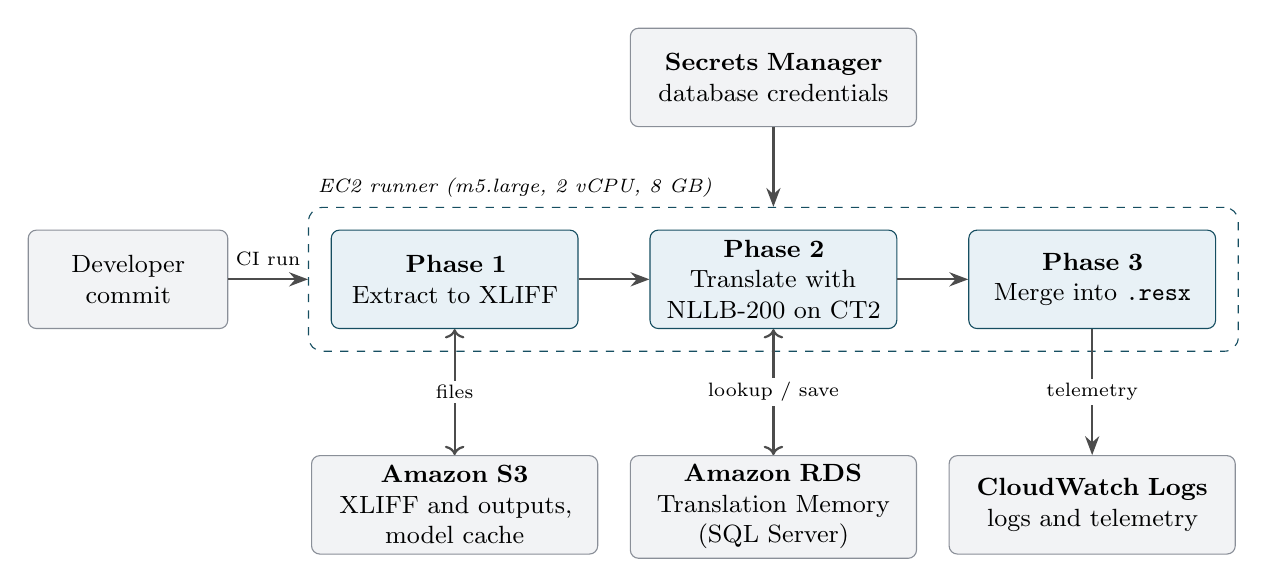
\begin{tikzpicture}[
  box/.style={draw=cnew!70!black, fill=boxblue, rounded corners=3pt, align=center, font=\small, minimum height=1.25cm, text width=2.9cm},
  src/.style={draw=cgrey, fill=boxgrey, rounded corners=3pt, align=center, font=\small, minimum height=1.25cm, text width=2.3cm},
  store/.style={draw=cgrey, fill=boxgrey, rounded corners=3pt, align=center, font=\small, minimum height=1.25cm, text width=3.4cm},
  arr/.style={-{Stealth[length=2.4mm]}, thick, draw=black!70},
  lbl/.style={font=\scriptsize, fill=white, inner sep=1.5pt}
]
\node[box] (p1) {\textbf{Phase 1}\\Extract to XLIFF};
\node[box, right=0.9cm of p1] (p2) {\textbf{Phase 2}\\Translate with\\NLLB-200 on CT2};
\node[box, right=0.9cm of p2] (p3) {\textbf{Phase 3}\\Merge into \code{.resx}};
\node[src, left=1.3cm of p1] (commit) {Developer\\commit};
\node[store, below=1.6cm of p1] (s3) {\textbf{Amazon S3}\\XLIFF and outputs,\\model cache};
\node[store, below=1.6cm of p2] (rds) {\textbf{Amazon RDS}\\Translation Memory\\(SQL Server)};
\node[store, below=1.6cm of p3] (cw) {\textbf{CloudWatch Logs}\\logs and telemetry};
\node[store, above=1.3cm of p2] (sm) {\textbf{Secrets Manager}\\database credentials};
\begin{scope}[on background layer]
\node[draw=cnew!70!black, dashed, rounded corners=5pt, fit=(p1)(p2)(p3), inner sep=8pt] (runner) {};
\end{scope}
\node[font=\scriptsize\itshape, anchor=south west] at (runner.north west) {EC2 runner (m5.large, 2 vCPU, 8 GB)};
\draw[arr] (commit) -- node[lbl, above=3pt]{CI run} (p1.west -| runner.west);
\draw[arr] (p1) -- (p2);
\draw[arr] (p2) -- (p3);
\draw[arr, <->] (p1) -- node[lbl]{files} (s3);
\draw[arr, <->] (p2) -- node[lbl]{lookup / save} (rds);
\draw[arr] (p3) -- node[lbl]{telemetry} (cw);
\draw[arr] (sm) -- (sm |- runner.north);
\end{tikzpicture}
\caption[The localization pipeline on AWS]{The localization pipeline on AWS. All resources are created by one
CloudFormation stack in \code{ap-south-1}.}
\label{fig:arch}
\end{figure}

\subsection{Azure to AWS Service Mapping}
The move to AWS changed only the services around the translation code (Table~\ref{tab:mapping}). The translation logic
itself was kept identical to the Azure version, and automated parity tests compare the two code bases so that any
divergence is a deliberate, documented change.

\begin{table}[H]
\centering
\caption[Azure to AWS service mapping]{Azure services of the previous semester and their AWS replacements.}
\label{tab:mapping}
\begin{tabularx}{\linewidth}{@{}l l L@{}}
\toprule
\textbf{Role} & \textbf{Azure (previous semester)} & \textbf{AWS (this semester)} \\
\midrule
File storage & Blob Storage & Amazon S3 (\code{runs/<run-id>/raw}, \code{translated}, \code{output}) \\
Translation Memory & Azure SQL Database & Amazon RDS for SQL Server Express \\
Telemetry & Application Insights & Amazon CloudWatch Logs (same \code{RESEARCH\_DATA} payload) \\
Credentials & pipeline variables & AWS Secrets Manager (RDS-managed password) \\
CI/CD orchestration & Azure DevOps Pipelines & EC2 runner driven by SSM Run Command$^{\dagger}$ \\
Infrastructure & manual set-up & AWS CloudFormation (one stack) \\
\bottomrule
\end{tabularx}

\smallskip
{\footnotesize $^{\dagger}$An AWS CodePipeline/CodeBuild definition is included, but CodeBuild is not enabled for this
account, so runs use an EC2 runner with the same three phases.}
\end{table}

\subsection{Baseline on AWS}
The first complete AWS run (\code{ec2-20261015t233954z}) translated the previous semester's 50-string workload into seven
languages with an empty memory. All seven files completed with no failures (Table~\ref{tab:awsbaseline}). This run is the
starting point for the profiling in Chapter~\ref{sec:profiling}.

\begin{table}[H]
\centering
\caption[First AWS run]{First AWS run: 50 strings per language, empty Translation Memory, beam 5 (m5.large, 2 cores).}
\label{tab:awsbaseline}
\begin{tabular}{@{}l S[table-format=2.2] S[table-format=4.0] S[table-format=2.2]@{}}
\toprule
\textbf{Language} & {\textbf{File time (s)}} & {\textbf{Strings/hour}} & {\textbf{Model time (s)}} \\
\midrule
de-DE & 22.30 & 8070 & 22.15 \\
es-ES & 21.19 & 8492 & 21.04 \\
fr-FR & 22.73 & 7920 & 22.59 \\
hi-IN & 21.71 & 8291 & 21.57 \\
ja-JP & 20.41 & 8820 & 20.27 \\
ru-RU & 22.10 & 8143 & 21.97 \\
zh-CN & 19.47 & 9247 & 19.32 \\
\midrule
\textbf{Average} & \bfseries 21.42 & \bfseries 8426 & \bfseries 21.27 \\
\bottomrule
\end{tabular}
\end{table}

\section{Datasets and Evaluation Setup}
\label{sec:setup}

\subsection{Datasets}
Three workloads were used (Table~\ref{tab:datasets}). The main results use the KDE4 corpus~\cite{opus}, a collection of
real user-interface strings from the KDE desktop software, prepared by the Track~1 team with reference translations in
twelve languages.

\begin{table}[H]
\centering
\caption[Datasets]{Datasets used in this report.}
\label{tab:datasets}
\begin{tabularx}{\linewidth}{@{}l l L@{}}
\toprule
\textbf{Dataset} & \textbf{Size} & \textbf{Used for} \\
\midrule
\code{.resx} workload & 3 files, 153 strings, 7 languages (1,071 translations) & first batching benchmark \\
FLORES-200 dev~\cite{nllb} & first 40 sentences, 7 languages & quality check of beam sizes \\
\textbf{KDE4} & 10,231 rows $\rightarrow$ \textbf{10,054 usable} strings, 12 languages & all main results \\
\bottomrule
\end{tabularx}
\end{table}

\paragraph{KDE4 preparation.} The twelve target languages are Hindi (hi), Arabic (ar), Bengali (bn), German (de),
Spanish (es), French (fr), Japanese (ja), Marathi (mr), Punjabi (pa), Tamil (ta), Telugu (te) and Chinese (zh). Of the
10,231 rows, 177 were removed: one cell containing hundreds of strings joined by line breaks, two cells that the
spreadsheet had converted to Boolean values, and duplicated English strings. The usable strings are short (median 13
characters, about two words), typical of user-interface text. 355 of them contain placeholders such as \code{\%1},
\code{\%s}, \code{\{name\}} or \code{<b>}.

\paragraph{Reference translations.} Several signs suggest that the KDE4 reference translations were produced by machine
rather than by KDE's human translators: every row is filled in all twelve languages, ``TRUE/FALSE'' appears as
``WAHR/FALSCH'', and the references themselves drop \code{\%N} placeholders in 5--25\% of rows. chrF in this report
therefore measures closeness to these references. Comparisons \emph{between} pipeline versions remain fair, because all
versions are scored against the same references; the placeholder measure does not use the references at all.

\subsection{Machine and Software}
All measurements ran on the same AWS instance type: \textbf{m5.large} (2 vCPU Intel Xeon Platinum 8259CL, 8 GB RAM,
on-demand price \$0.101 per hour in \code{ap-south-1}). The translation container is pinned to the machine's two cores.
The model is \code{facebook/nllb-200-distilled-600M}, converted to CTranslate2 4.7.1 with INT8 weights.

\subsection{Measures}
\begin{table}[H]
\centering
\caption[Measures]{Measures reported in this report.}
\label{tab:measures}
\begin{tabularx}{\linewidth}{@{}l L@{}}
\toprule
\textbf{Measure} & \textbf{Meaning} \\
\midrule
Time, translations/hour & wall-clock time of the measured stage, and its throughput \\
Speed-up & time of the reference configuration divided by time of the new one \\
Model tokens & real tokens read and written by the model (tokenizer counts) \\
Padding & share of the model's input positions filled with padding inside batches \\
CPU busy & CPU time used divided by wall time $\times$ available cores \\
chrF & character n-gram F-score~\cite{chrf} against the reference translations, computed with SacreBLEU~\cite{sacrebleu} (0--100, higher is better) \\
BLEU & word n-gram precision score against the references (SacreBLEU \code{13a}; Chinese \code{zh}; Japanese MeCab) \\
spBLEU & BLEU on FLORES-200 SentencePiece pieces~\cite{flores}, comparable across scripts \\
COMET & neural quality estimate (\code{Unbabel/wmt22-comet-da}~\cite{comet}, 0--1) on the same 1,000 random strings in every language \\
Placeholders kept & share of strings with placeholders whose output contains exactly the same placeholders \\
Cost & machine time $\times$ on-demand price \\
\bottomrule
\end{tabularx}
\end{table}

\subsection{Method}
Every optimization was evaluated \textbf{one change at a time}, starting from the best configuration found so far, so that
each gain can be traced to its cause. Changes that should not alter the output (batch layout, parallelism, length caps)
were checked for \textbf{identical translations}. Changes that do alter the output (beam size, placeholder handling,
translation reuse) were scored for quality before being adopted.

\section{Baseline Profiling}
\label{sec:profiling}

The telemetry of the first AWS run (Table~\ref{tab:awsbaseline}) splits each file's time into its parts. On average a
50-string file took 21.42~s, of which \textbf{21.27~s (99.3\%) was model inference}. Database lookups, S3 transfers and
XML processing together took about 0.15~s. Any meaningful speed-up therefore has to come from the model stage: either
making each model call cheaper, or making fewer of them.

\subsection{How Batching Worked}
Phase~2 processed one file and one language at a time. It filled a batch with untranslated strings in file order until
the batch held 52 strings or an \emph{estimated} 1,024 tokens (characters divided by four), sent it to the model with
beam size~5 (five candidate translations per string), and waited for the result before sending the next batch.

\subsection{Flaws Found}
\begin{table}[H]
\centering
\caption[Flaws of the original batching]{Flaws of the original batching logic, and the evidence for each.}
\label{tab:flaws}
\begin{tabularx}{\linewidth}{@{}l L@{}}
\toprule
\textbf{Flaw} & \textbf{Evidence} \\
\midrule
Guessed token counts & batches were cut by characters $\div$ 4, not by the tokens the model actually reads \\
Mixed-length batches & short and long strings shared batches; \textbf{30\%} of the model's input positions were padding \\
One batch at a time & only one batch was in the engine at any moment; the two cores were \textbf{59\%} busy on average \\
Five candidates per string & beam~5 decodes five hypotheses for every string, the dominant cost (Chapter~\ref{sec:batching}) \\
No output limit & a single string with an unusually long output could hold up its whole batch \\
\bottomrule
\end{tabularx}
\end{table}

\keyresult{\textbf{RQ1.} Model inference accounts for 99.3\% of the translation stage. Within it, the original batching
wasted input positions on padding (30\%), left part of the CPU idle (59\% busy) and paid for five candidate translations
per string.}

\section{Batching Optimization}
\label{sec:batching}

Batching decides how strings are grouped before they reach the model. This chapter tests each part of the batching logic
separately: batch layout and sorting, beam size, and parallel execution with an output length cap.

\subsection{Benchmark Method}
A benchmark tool runs inside the production container, with the same model, the same two pinned cores and the same
machine type, and times only model inference (tokenize, translate, detokenize). Its baseline step calls the production
translation function itself, and a sanity check confirmed that the benchmark engine reproduces production output exactly
(100 of 100 strings).

\subsection{Batch Layout and Sorting}
Table~\ref{tab:layout} applies the layout changes to the \code{.resx} workload (1,071 translations). A run-wide plan with
real token counts and 1,024-token batches, sorted by length, cut padding from 30.1\% to 4.3\%. Smaller and larger token
budgets were also tested.

\begin{table}[H]
\centering
\caption[Batch layout and beam size]{Batch layout and beam size on the \code{.resx} workload (run
\code{ec2-20261016t103748z}). ``Identical'' compares the output with the baseline's output.}
\label{tab:layout}
\small\setlength{\tabcolsep}{4.5pt}
\begin{tabular}{@{}l l c S[table-format=3.2] S[table-format=1.2] S[table-format=2.1] c c@{}}
\toprule
\textbf{Step} & \textbf{Change} & \textbf{Beam} & {\textbf{Time (s)}} & {\textbf{Speed-up}} & {\textbf{Padding (\%)}} & \textbf{Peak mem.} & \textbf{Identical} \\
\midrule
A & Original pipeline & 5 & 434.84 & 1.00 & 30.1 & 1.8 GB & -- \\
D-256 & Sorted, 256-token batches & 5 & 451.10 & 0.96 & 1.2 & 1.8 GB & 100\% \\
D-512 & Sorted, 512-token batches & 5 & 432.62 & 1.01 & 2.4 & 2.2 GB & 100\% \\
D-1024 & Sorted, 1,024-token batches & 5 & 425.78 & 1.02 & 4.3 & 3.5 GB & 100\% \\
\midrule
F & D-1024 + beam 2 & 2 & 188.08 & 2.31 & 4.3 & 3.5 GB & 77\% \\
G & D-1024 + beam 1 & 1 & 103.58 & 4.20 & 4.3 & 3.5 GB & 59\% \\
\bottomrule
\end{tabular}
\end{table}

\begin{figure}[H]
\centering
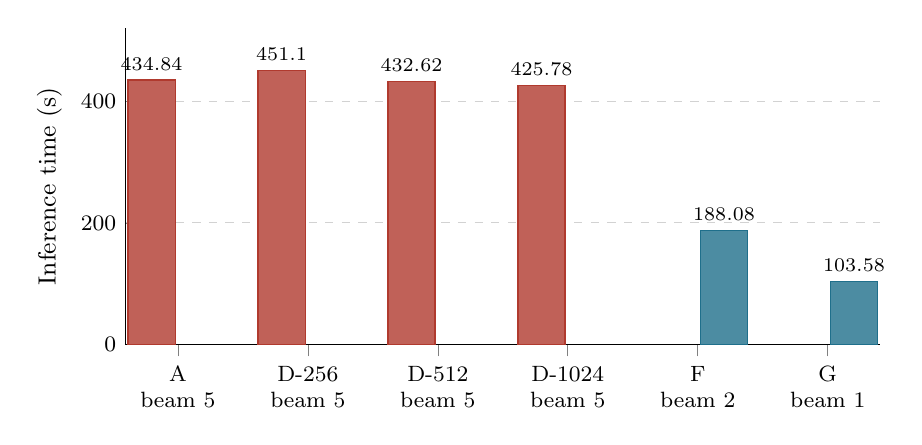
\begin{tikzpicture}
\begin{axis}[reportbars, width=0.92\linewidth, height=5.6cm, bar width=17pt,
  symbolic x coords={A,D-256,D-512,D-1024,F,G}, xtick={A,D-256,D-512,D-1024,F,G},
  ylabel={Inference time (s)}, ymin=0, ymax=520,
  nodes near coords, nodes near coords align={vertical},
  xticklabels={{A\\beam 5},{D-256\\beam 5},{D-512\\beam 5},{D-1024\\beam 5},{F\\beam 2},{G\\beam 1}},
  xticklabel style={align=center}]
\addplot[fill=cprev!80, draw=cprev] coordinates {(A,434.84) (D-256,451.10) (D-512,432.62) (D-1024,425.78)};
\addplot[fill=cnew!80, draw=cnew] coordinates {(F,188.08) (G,103.58)};
\end{axis}
\end{tikzpicture}
\caption[Inference time per batching step]{Inference time for each batching step. Layout changes (red) moved time by at
most 4\%; beam size (blue) halved it or more.}
\label{fig:layout}
\end{figure}

\paragraph{Finding.} Layout changes never altered a translation, but moved time by only $-4\%$ to $+2\%$, within the
2\% run-to-run noise measured on identical work. Padding fell from 30\% to 1--4\% without a matching speed-up:
\textbf{padding is not the bottleneck}. Peak memory, however, roughly doubled with 1,024-token batches, and a 4,096-token
attempt did not complete on the 8~GB machine, so batches above about 1,024 tokens were ruled out. Telling CTranslate2
explicitly to use two threads per batch also changed nothing.

\subsection{Beam Size}
The beam size is the number of candidate translations the model keeps while decoding. Steps F and G show that it, not
the layout, dominates the cost: beam~2 was 2.31\x{} and beam~1 4.20\x{} faster than the baseline. Because a smaller
beam changes the output, quality was checked on two datasets.

\paragraph{FLORES-200.} On 40 human-translated sentences per language (Table~\ref{tab:flores}), beam~2 lost 0.87 chrF and
beam~1 lost 1.40 chrF overall.

\begin{table}[H]
\centering
\caption[chrF on FLORES-200 by beam size]{chrF on FLORES-200 (first 40 dev sentences per language) by beam size.}
\label{tab:flores}
\begin{tabular}{@{}c S[table-format=2.2] *{7}{S[table-format=2.2]}@{}}
\toprule
\textbf{Beam} & {\textbf{All 7}} & {de-DE} & {es-ES} & {fr-FR} & {hi-IN} & {ja-JP} & {ru-RU} & {zh-CN} \\
\midrule
5 & 56.69 & 62.71 & 55.54 & 68.75 & 57.65 & 33.83 & 58.35 & 28.58 \\
2 & 55.82 & 61.93 & 55.63 & 67.05 & 56.98 & 34.77 & 56.71 & 26.32 \\
1 & 55.29 & 60.08 & 55.73 & 67.76 & 55.03 & 33.39 & 57.33 & 25.07 \\
\bottomrule
\end{tabular}
\end{table}

\paragraph{KDE4.} Forty sentences per language is a small sample, so the comparison was repeated on a fixed random sample
of 1,000 KDE4 strings in all twelve languages (12,000 translations per beam), using run-wide, length-sorted 1,024-token
batches (Tables~\ref{tab:kde4beam} and~\ref{tab:kde4beamlang}).

\begin{table}[H]
\centering
\caption[Beam size on the KDE4 sample]{Beam size on 1,000 KDE4 strings $\times$ 12 languages (run \code{ec2-20261016t115802z}).}
\label{tab:kde4beam}
\begin{tabular}{@{}c S[table-format=4.0] S[table-format=5.0] S[table-format=1.2] S[table-format=2.2] c@{}}
\toprule
\textbf{Beam} & {\textbf{Time (s)}} & {\textbf{Translations/hour}} & {\textbf{Speed-up}} & {\textbf{chrF (all 12)}} & \textbf{Identical to beam 5} \\
\midrule
5 & 3169 & 13631 & 1.00 & 64.41 & -- \\
\textbf{2} & \bfseries 1442 & \bfseries 29949 & \bfseries 2.20 & \bfseries 63.96 & 84\% \\
1 & 915 & 47197 & 3.46 & 62.26 & 69\% \\
\bottomrule
\end{tabular}
\end{table}

\begin{table}[H]
\centering
\caption[chrF per language by beam size]{chrF per language on the KDE4 sample by beam size.}
\label{tab:kde4beamlang}
\small
\begin{tabular}{@{}c *{12}{S[table-format=2.2]}@{}}
\toprule
\textbf{Beam} & {hi} & {ar} & {bn} & {de} & {es} & {fr} & {ja} & {mr} & {pa} & {ta} & {te} & {zh} \\
\midrule
5 & 66.90 & 57.15 & 64.87 & 65.06 & 72.01 & 70.23 & 53.43 & 59.34 & 63.35 & 64.70 & 66.07 & 39.68 \\
2 & 66.61 & 55.74 & 64.11 & 64.39 & 71.69 & 69.48 & 52.52 & 59.08 & 63.27 & 65.07 & 65.86 & 39.30 \\
1 & 65.60 & 53.77 & 63.88 & 62.21 & 68.49 & 68.16 & 46.51 & 58.76 & 62.68 & 63.70 & 64.26 & 33.72 \\
\bottomrule
\end{tabular}
\end{table}

\begin{figure}[H]
\centering
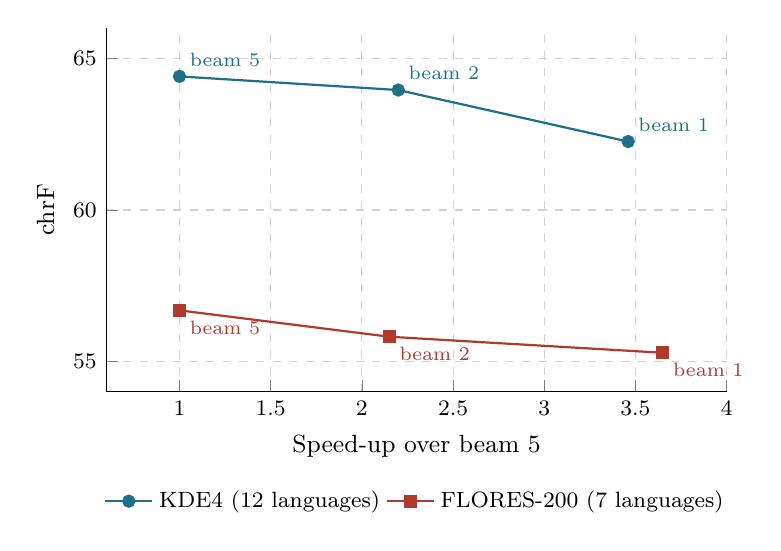
\begin{tikzpicture}
\begin{axis}[width=0.78\linewidth, height=6.2cm, axis lines*=left, ymajorgrids, xmajorgrids, grid style={dashed,gray!35},
  xlabel={Speed-up over beam 5}, ylabel={chrF}, xmin=0.6, xmax=4.0, ymin=54, ymax=66,
  tick label style={font=\footnotesize}, label style={font=\small},
  legend style={font=\footnotesize, draw=none, legend columns=2, at={(0.5,-0.24)}, anchor=north}]
\addplot[mark=*, thick, color=cnew, nodes near coords, point meta=explicit symbolic,
  every node near coord/.append style={font=\scriptsize, anchor=south west}]
  coordinates {(1.00,64.41)[beam 5] (2.20,63.96)[beam 2] (3.46,62.26)[beam 1]};
\addlegendentry{KDE4 (12 languages)}
\addplot[mark=square*, thick, color=cprev, nodes near coords, point meta=explicit symbolic,
  every node near coord/.append style={font=\scriptsize, anchor=north west}]
  coordinates {(1.00,56.69)[beam 5] (2.15,55.82)[beam 2] (3.65,55.29)[beam 1]};
\addlegendentry{FLORES-200 (7 languages)}
\end{axis}
\end{tikzpicture}
\caption[Speed against quality by beam size]{Speed against quality for beam sizes 5, 2 and 1. Beam 2 keeps almost all
of the quality at more than twice the speed.}
\label{fig:beam}
\end{figure}

\paragraph{Finding.} On real localization text, beam~2 is \textbf{2.2\x{} faster for a 0.45-point chrF loss}, and every
language stays within 1.4 points of beam~5 (Tamil slightly improves). Beam~1 costs more on KDE4 than on FLORES, with large
drops for Japanese ($-6.9$) and Chinese ($-6.0$), which makes it unsuitable for these languages. Beam~2 was adopted for
production.

\subsection{Parallel Batches and an Output Length Cap}
During the KDE4 runs the machine's CPU was only about 59\% busy: CTranslate2 processed one batch at a time and part of the
two cores sat idle. Three steps were tested on 500 KDE4 strings in 12 languages (6,000 translations, beam~2):

\begin{itemize}
  \item \textbf{P1:} load the model with two engine workers (\code{inter\_threads=2}, \code{intra\_threads=1}) and queue all
        batches at once, so two batches are translated in parallel, one per core.
  \item \textbf{P2:} P1 with smaller 512-token batches.
  \item \textbf{P3:} P1 plus a per-batch output cap of twice the longest input plus 10 tokens. Because batches are sorted by
        length, the cap fits every string in the batch and only stops runaway outputs.
\end{itemize}

\begin{table}[H]
\centering
\caption[Parallel batches and output length cap]{Parallel batches and output length cap (run \code{ec2-20261016t142418z}, 6,000 translations, beam 2).}
\label{tab:parallel}
\begin{tabular}{@{}l l S[table-format=3.2] S[table-format=1.2] S[table-format=2.1] c c@{}}
\toprule
\textbf{Step} & \textbf{Change} & {\textbf{Time (s)}} & {\textbf{Speed-up}} & {\textbf{CPU busy (\%)}} & \textbf{Identical} & \textbf{Peak mem.} \\
\midrule
P0 & One batch at a time & 617.52 & 1.00 & 59.3 & -- & 2.6 GB \\
P1 & Two batches in parallel & 514.97 & 1.20 & 99.6 & 100\% & 4.5 GB \\
P2 & P1 with 512-token batches & 539.68 & 1.14 & 99.3 & 99.9\% & 4.5 GB \\
\textbf{P3} & \textbf{P1 + output length cap} & \bfseries 488.14 & \bfseries 1.27 & 99.6 & \textbf{100\%} & 4.5 GB \\
\bottomrule
\end{tabular}
\end{table}

\paragraph{Finding.} Parallel batches raised CPU use from 59\% to 99.6\% and made translation 1.20\x{} faster with
identical output. The gain is below 2\x{} because two cores sharing the work each run slower than one core alone, and
it costs a second set of working buffers (2.6 to 4.5~GB, still safe on 8~GB). Smaller batches were slower, because more
batches mean more per-batch overhead. The length cap added a further 6\% (1.27\x{} in total) without changing a single
translation.

\subsection{Adopted Configuration}
\begin{table}[H]
\centering
\caption[Adopted batching configuration]{Batching configuration before and after this chapter.}
\label{tab:adopted}
\begin{tabularx}{\linewidth}{@{}l L L@{}}
\toprule
\textbf{Setting} & \textbf{Before} & \textbf{After} \\
\midrule
Order of strings & file order & sorted by length within each file, in chunks of 1,000 strings \\
Batch size & 52 strings or $\sim$1,024 \emph{estimated} tokens & up to 1,024 \emph{real} tokens \\
Execution & one batch at a time & all batches of a chunk queued, two engine workers \\
Output length & unlimited & 2 $\times$ longest input + 10 tokens per batch \\
Beam size & 5 & 2 \\
\bottomrule
\end{tabularx}
\end{table}

\keyresult{\textbf{RQ2.} Padding and batch layout are not the bottleneck: cutting padding from 30\% to 4\% gained 3\%.
The real levers are the beam size (2.2\x{} for $-0.45$ chrF on KDE4) and keeping both cores busy (1.27\x{} with identical
output). Together these are about 2.8\x{} faster in the benchmark.}

\section{Placeholder Protection}
\label{sec:placeholders}

Software strings contain placeholders that the program fills in at run time, such as \code{\%1}, \code{\%s},
\code{\{name\}} or \code{<b>}. A translation that drops or alters a placeholder is not merely a lower-quality translation:
it produces a broken message in the released software.

\subsection{The Problem}
In the KDE4 beam study, about \textbf{12\% of strings with placeholders} came back with a placeholder missing or changed,
at every beam size (88.0\% kept at beam~5, 87.7\% at beam~2). The model treats \code{\%1} as ordinary text and sometimes
translates, moves or drops it. Because beam size barely affected the problem, it needed its own fix.

\subsection{Method}
Before translation, each placeholder is replaced by a numbered marker; after translation the markers are replaced by the
original placeholders. The restore step accepts what the model does to a marker in practice (full-width brackets in
Chinese and Japanese, spaces inside the marker, digits written in the target script) and reports whether every marker
came back exactly once. If not, the string is translated again without markers and that result is used (the
\emph{fallback}). Three marker styles were compared on all 355 KDE4 placeholder strings in 12 languages (4,260
translations per style, beam~2):

\begin{center}
\small
\begin{tabular}{@{}l l@{}}
\code{Could not find conduit \%1.} & original \\
\code{Could not find conduit [0].} & square \\
\code{Could not find conduit \S0\S.} & section \\
\code{Could not find conduit \{0\}.} & curly \\
\end{tabular}
\end{center}

\subsection{Results}
\begin{table}[H]
\centering
\caption[Placeholder survival by marker style]{Placeholder survival by marker style (run \code{ec2-20261016t195057z}, 4,260 translations per style).}
\label{tab:phstyles}
\begin{tabular}{@{}l S[table-format=2.2] S[table-format=2.2] S[table-format=2.2] S[table-format=3.1]@{}}
\toprule
\textbf{Style} & {\textbf{Kept (\%)}} & {\textbf{Kept with fallback (\%)}} & {\textbf{Fallback used (\%)}} & {\textbf{Time (s)}} \\
\midrule
None (before) & 87.70 & {--} & {--} & 649.3 \\
\textbf{Square} \code{[0]} & \bfseries 99.15 & \bfseries 99.88 & 0.85 & 716.1 \\
Section \code{\S0\S} & 80.66 & 97.91 & 19.34 & 749.5 \\
Curly \code{\{0\}} & 88.78 & 97.37 & 11.22 & 747.8 \\
\bottomrule
\end{tabular}
\end{table}

\begin{figure}[H]
\centering
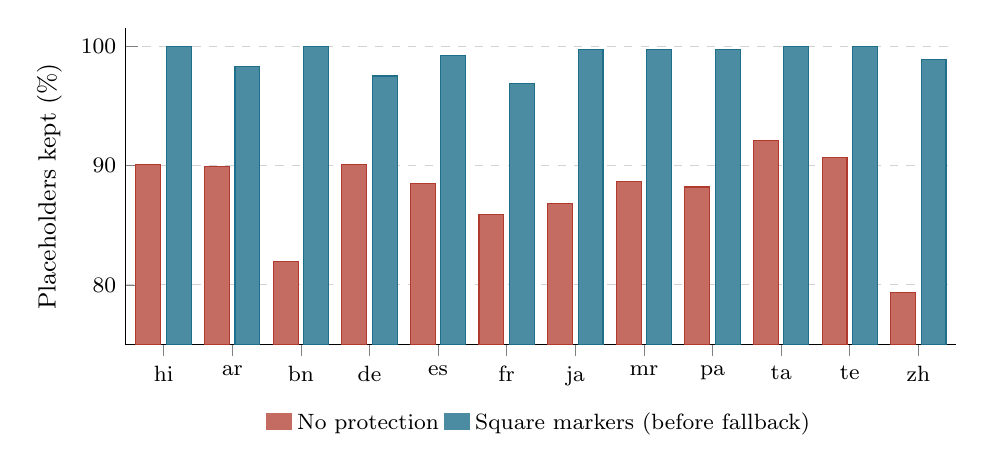
\begin{tikzpicture}
\begin{axis}[reportbars, width=\linewidth, height=5.6cm, bar width=9pt,
  symbolic x coords={hi,ar,bn,de,es,fr,ja,mr,pa,ta,te,zh}, xtick=data,
  ylabel={Placeholders kept (\%)}, ymin=75, ymax=101.5, enlarge x limits=0.05]
\addplot[fill=cprev!75, draw=cprev] coordinates {(hi,90.1) (ar,89.9) (bn,82.0) (de,90.1) (es,88.5) (fr,85.9) (ja,86.8) (mr,88.7) (pa,88.2) (ta,92.1) (te,90.7) (zh,79.4)};
\addplot[fill=cnew!80, draw=cnew] coordinates {(hi,100) (ar,98.3) (bn,100) (de,97.5) (es,99.2) (fr,96.9) (ja,99.7) (mr,99.7) (pa,99.7) (ta,100) (te,100) (zh,98.9)};
\legend{No protection, Square markers (before fallback)}
\end{axis}
\end{tikzpicture}
\caption[Placeholders kept per language]{Placeholders kept per language, without protection and with square markers.
Chinese improves the most (79.4\% to 98.9\%).}
\label{fig:placeholders}
\end{figure}

\paragraph{Finding.} Square markers raise placeholder survival from \textbf{87.7\% to 99.15\%}, and to \textbf{99.88\%}
with the fallback: 5 broken strings out of 4,260 instead of about 524. Every language reaches at least 96.9\% before the
fallback. The square style works because NLLB saw many citation markers such as \code{[1]} during training and copies
them unchanged; it often rewrites the other two styles. The cost is about 10\% more time on strings with placeholders,
which are 3.5\% of KDE4, so the overall effect is negligible. Square markers with the fallback were adopted.

\paragraph{Note on chrF.} On these 355 strings, chrF against the references fell by about two points (61.79 to 59.76 with
fallback). The likely cause is that the references themselves drop \code{\%N} placeholders in 5--25\% of rows, so a
translation that correctly keeps them matches those references less closely. Strings without placeholders are not
affected by protection.

\section{Full KDE4 Production Run}
\label{sec:kde4run}

The benchmarks in Chapters~\ref{sec:batching} and~\ref{sec:placeholders} timed the model alone on samples of up to 1,000
strings. This chapter puts all the changes into the \textbf{production pipeline} (Phases~1--3, Translation Memory, S3,
telemetry) and translates the \textbf{whole KDE4 dataset}.

\subsection{Setup}
All 10,054 usable KDE4 strings were packed into one \code{.resx} file and translated into all 12 languages:
\textbf{120,648 translations}. The pipeline used the adopted batching configuration (Table~\ref{tab:adopted}), beam~2 and
placeholder protection, on the same m5.large. The Translation Memory was emptied first, so every string went through the
model (run \code{ec2-20261016t214343z}).

\subsection{Results}
The run succeeded: 12 of 12 language files, \textbf{0 failures, 0 missing strings}.

\begin{table}[H]
\centering
\caption[Full KDE4 run per language: speed]{Full KDE4 run per language: speed and placeholder survival, 10,054 strings per language.}
\label{tab:kde4run}
\begin{tabular}{@{}l S[table-format=2.2] S[table-format=5.0] S[table-format=3.2]@{}}
\toprule
\textbf{Language} & {\textbf{Time (min)}} & {\textbf{Translations/hour}} & {\textbf{Placeholders kept (\%)}} \\
\midrule
Arabic (ar) & 18.28 & 32991 & 99.72 \\
Bengali (bn) & 18.38 & 32828 & 100.00 \\
German (de) & 17.83 & 33841 & 99.44 \\
Spanish (es) & 17.62 & 34232 & 100.00 \\
French (fr) & 19.00 & 31742 & 99.72 \\
Hindi (hi) & 16.12 & 37429 & 100.00 \\
Japanese (ja) & 16.18 & 37282 & 100.00 \\
Marathi (mr) & 17.02 & 35434 & 100.00 \\
Punjabi (pa) & 19.30 & 31258 & 100.00 \\
Tamil (ta) & 18.77 & 32144 & 100.00 \\
Telugu (te) & 19.15 & 31502 & 100.00 \\
Chinese (zh) & 16.73 & 36059 & 99.72 \\
\midrule
\textbf{All} & \bfseries 214.4 & \bfseries 33760 & \bfseries 99.88 \\
\bottomrule
\end{tabular}
\end{table}

\begin{table}[H]
\centering
\caption[Translation quality of the full KDE4 run]{Translation quality of the full KDE4 run. chrF, BLEU and spBLEU use
all 10,054 strings per language; COMET uses the same fixed sample of 1,000 strings in every language.}
\label{tab:kde4quality}
\begin{tabular}{@{}l S[table-format=2.2] S[table-format=2.2] S[table-format=2.2] S[table-format=1.4]@{}}
\toprule
\textbf{Language} & {\textbf{chrF}} & {\textbf{BLEU}} & {\textbf{spBLEU}} & {\textbf{COMET}} \\
\midrule
Arabic (ar) & 55.42 & 32.45 & 39.44 & 0.8296 \\
Bengali (bn) & 64.38 & 37.38 & 52.52 & 0.8866 \\
German (de) & 64.22 & 39.92 & 45.88 & 0.8639 \\
Spanish (es) & 71.50 & 50.65 & 53.15 & 0.8704 \\
French (fr) & 68.89 & 44.18 & 46.65 & 0.8495 \\
Hindi (hi) & 64.75 & 43.24 & 49.75 & 0.8526 \\
Japanese (ja) & 50.92 & 32.35 & 39.07 & 0.8643 \\
Marathi (mr) & 58.45 & 35.76 & 44.38 & 0.8249 \\
Punjabi (pa) & 61.53 & 38.56 & 50.42 & 0.8689 \\
Tamil (ta) & 64.10 & 37.75 & 49.53 & 0.8840 \\
Telugu (te) & 65.28 & 40.85 & 53.82 & 0.8932 \\
Chinese (zh) & 39.84 & 42.48 & 42.55 & 0.8530 \\
\midrule
\textbf{All} & \bfseries 63.29 & {\bfseries 39.63$^{\ast}$} & \bfseries 47.90 & \bfseries 0.8617 \\
\bottomrule
\end{tabular}

\smallskip
{\footnotesize $^{\ast}$Mean of the 12 languages: BLEU uses different word splitting for Chinese and Japanese, so a single
corpus score across languages is not meaningful. spBLEU uses the same pieces for every language.}
\end{table}

\begin{figure}[H]
\centering
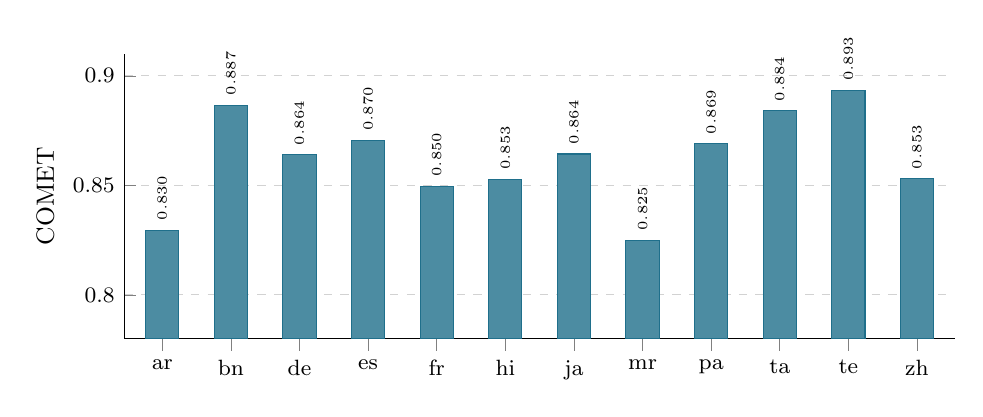
\begin{tikzpicture}
\begin{axis}[reportbars, width=\linewidth, height=5.2cm, bar width=12pt,
  symbolic x coords={ar,bn,de,es,fr,hi,ja,mr,pa,ta,te,zh}, xtick=data,
  ylabel={COMET}, ymin=0.78, ymax=0.91, enlarge x limits=0.05,
  yticklabel style={/pgf/number format/fixed, /pgf/number format/precision=2},
  nodes near coords, nodes near coords style={font=\tiny, rotate=90, anchor=west, /pgf/number format/fixed, /pgf/number format/fixed zerofill, /pgf/number format/precision=3}]
\addplot[fill=cnew!80, draw=cnew] coordinates {(ar,0.8296) (bn,0.8866) (de,0.8639) (es,0.8704) (fr,0.8495) (hi,0.8526) (ja,0.8643) (mr,0.8249) (pa,0.8689) (ta,0.8840) (te,0.8932) (zh,0.8530)};
\end{axis}
\end{tikzpicture}
\caption[COMET per language in the full KDE4 run]{COMET per language in the full KDE4 run (1,000-string sample per
language). Every language lies between 0.82 and 0.90.}
\label{fig:kde4chrf}
\end{figure}

\paragraph{Reading the metrics together.} The four metrics agree on most languages, with one exception. chrF places
Chinese far below every other language (39.84), but BLEU (42.48), spBLEU (42.55) and COMET (0.853) put it in the middle.
chrF compares sequences of up to six characters, which is harsh for Chinese, where a word is often one or two
characters; COMET, which judges meaning with a neural model, is the fairer comparison across scripts.

\paragraph{Where the time goes.} Translation took \textbf{3~h~34~min} (3~h~38~min for the whole run, including model
loading and Phases~1 and~3). Model inference accounted for 99.6\% of Phase~2; Translation Memory reads and writes took
about 44~s in total, and XML and S3 a few seconds. During translation the machine's CPU was 92--100\% busy, and memory use
stayed at 1.6--1.9~GB per file.

\subsection{Comparison with the Starting Configuration}
The starting configuration (beam~5, one batch at a time) ran at 13,631 translations per hour in the KDE4 benchmark
(Table~\ref{tab:kde4beam}). At that rate this dataset would take an estimated \textbf{8.9 hours}; the optimized
production pipeline needed \textbf{3.6 hours}, about \textbf{2.5\x{} faster}. The benchmarks predicted 2.8\x{}; the
difference is the work the benchmark does not time: tokenization, placeholder handling, XML, database saves, and the end
of each 1,000-string chunk, where only one batch is left for the two cores.

\keyresult{\textbf{RQ3.} The optimized pipeline translated the whole twelve-language KDE4 corpus (120,648 translations)
in 3.6 hours with no failures, at 33,760 translations per hour, with chrF 63.29, spBLEU 47.90, COMET 0.862 and
99.88\% of placeholders kept: about 2.5\x{} faster than the semester's starting configuration.}

\section{Quality Problems Found at Scale}
\label{sec:quality}

Translating the full corpus revealed two problems that the smaller tests could not show.

\subsection{Characters the Model Cannot Write}
Four strings in the full run came back \emph{empty}: \code{thistle} (Japanese) and \code{Candle}, \code{crab} and
\code{goy Y} (Chinese). Reproducing them with the same model showed the cause: for these strings the model's best output is
the \code{<unk>} (unknown) token, and decoding removes special tokens, leaving nothing. The behaviour is the same at beam~5
and unrelated to batching.

Re-translating the whole Chinese and Japanese sets showed that the empty strings were only the visible part. \textbf{614 of
10,054 Chinese outputs (6.1\%)} and 8 Japanese outputs contained \code{<unk>}. In most of them a character was silently
deleted and the meaning changed: ``New Folder'' became ``new file'', ``Dolphin
Toolbar'' became ``fish tool'', and ``Bitrate'' became just ``rate''.

\subsection{Options Measured}
Three ways of handling these strings were scored against the references on exactly the affected strings
(Table~\ref{tab:unk}).

\begin{table}[H]
\centering
\caption[Handling of \code{<unk>} outputs]{Handling of outputs that contain \code{<unk>} (chrF on the affected strings).}
\label{tab:unk}
\begin{tabularx}{\linewidth}{@{}l S[table-format=2.2] S[table-format=2.2] L@{}}
\toprule
\textbf{Option} & {\textbf{zh (614)}} & {\textbf{ja (8)}} & \textbf{Behaviour} \\
\midrule
Keep the model's text & 26.20 & 6.61 & characters silently missing; meaning often wrong \\
Forbid \code{<unk>} and retry & 25.97 & 33.18 & fixes some; others become ``??'' or a wrong word (``Tunnels'' $\rightarrow$ ``Tunisia'', ``thistle'' $\rightarrow$ ``carbohydrate'') \\
\textbf{Keep the English and report it} & 7.70 & 31.71 & never a wrong word; listed in the log for a translator \\
\bottomrule
\end{tabularx}
\end{table}

\paragraph{Decision.} The pipeline keeps such strings in English and reports them. In localized software, a visibly
untranslated string can be found and fixed; a wrong word cannot. The cost is a lower measured chrF for Chinese, since
chrF counts English as untranslated. Translation Memory entries for these strings are handled in
Chapter~\ref{sec:tmdesign}.

\subsection{Long Strings and the Translation Memory}
The Translation Memory used the English text itself as its database key. SQL Server limits a key to 900 bytes, which
allows at most 434 characters, while KDE4 contains strings of up to 660 characters; saving such a string failed. The key
is now a fixed-size \textbf{SHA-256 hash} of the text, and the text is stored in an unlimited column, so strings of any
length are saved and found again.

\subsection{Verification}
A check run (\code{ec2-20261017t063722z}) translated 383 KDE4 strings (the three longest, 25 known \code{<unk>} cases and
all 355 placeholder strings) in 12 languages, twice, as two identical files. All 24 files succeeded. The second copy was
served \textbf{100\% from the memory} in ten languages, including the long strings; the only misses were the Chinese and
Japanese strings kept in English, which were all listed in the log. Placeholder survival matched Chapter~\ref{sec:placeholders}.

\keyresult{\textbf{RQ4.} At scale, 6.1\% of Chinese outputs silently lost characters the model cannot write, and strings
over 434 characters could not be stored in the memory. Affected strings are now kept in English and reported, and the
memory is keyed by a hash so that strings of any length fit.}

\section{Translation Memory Redesign}
\label{sec:tmdesign}

A Translation Memory (TM) is a store of translations the pipeline has already made. Before sending a string to the model,
the pipeline looks it up; a \emph{hit} is reused instantly, and a \emph{miss} is translated and saved for next time. The
previous semester's memory worked, and measured a seeded 0\% versus 50\% cache. This chapter rebuilds it for the way the
pipeline is actually used: on every commit of an evolving application.

\subsection{Problems with the Previous Memory}
\begin{table}[H]
\centering
\caption[Problems of the previous memory]{Problems of the previous Translation Memory.}
\label{tab:tmflaws}
\begin{tabularx}{\linewidth}{@{}l L@{}}
\toprule
\textbf{Problem} & \textbf{Consequence} \\
\midrule
Emptied before every run & each commit retranslated the whole application, although a commit changes only a few strings \\
No check of which model made an entry & after a model or setting change, older translations would still be reused \\
One query per 1,000 strings per file & every file asked the database again for its own strings \\
Exact matches only & ``8 Cards'' could not reuse ``20 Cards''; 526 KDE4 strings (5.2\%) have such a near-twin \\
\bottomrule
\end{tabularx}
\end{table}

\subsection{Design}
\paragraph{Persistent, engine-labelled memory.} The memory is kept between runs. Each entry records its \emph{engine
version}: the model and every setting that changes the output (beam size, length cap, placeholder style, handling of
\code{<unk>}). Lookups match the current engine version, so a change of model or settings automatically stops older entries
from being reused, without deleting anything. The table key is (language, engine version, text hash), with the language
first so that one language's entries are stored together.

\paragraph{One load per language per run.} At the first file of a language, the pipeline loads that language's entries
for the current engine in a single query and keeps them in memory. Every later check is an in-process dictionary lookup,
and translations made during the run are added as they are saved, so later files reuse them without another query.

\paragraph{Near-twin reuse.} When the exact text is not found, the pipeline looks for a saved \emph{model} translation of a
string that differs only in numbers, placeholders or trailing punctuation, and adapts it:

\begin{center}
\small
\begin{tabular}{@{}l l l@{}}
\toprule
\textbf{Saved} & \textbf{New string} & \textbf{Adapted translation} \\
\midrule
\code{20 Cards} $\rightarrow$ \code{20 Karten} & \code{8 Cards} & \code{8 Karten} \\
\code{Copy \%1 to \%2} $\rightarrow$ \code{Nach \%2 kopieren: \%1} & \code{Copy \%3 to \%4} & \code{Nach \%4 kopieren: \%3} \\
\code{Border} $\rightarrow$ \code{Rahmen} & \code{Border:} & \code{Rahmen:} \\
\bottomrule
\end{tabular}
\end{center}

Reuse is refused, and the string goes to the model as usual, whenever it cannot be done cleanly: a value does not appear
exactly once in the saved translation (for example, the model wrote the number in local digits), the English repeats a
value (``1 of 1''), or the saved entry was itself adapted. Twins inside one file are sent to the model once and the rest
are adapted from that translation.

\subsection{Quality Check of Near-Twin Reuse}
Reuse only helps if adapted translations are as good as the model's own. Before enabling it, every twin pair in the full
KDE4 set (440 groups, 968 strings, 528 reusable pairs) was translated in all twelve languages both ways: freshly by the
production model and settings, and adapted from its twin. Both were scored against the references.

A first version \emph{guessed} how each language writes trailing punctuation and scored lower than fresh translation for
Japanese. Counting the endings of every KDE4 reference showed that only Chinese consistently uses the full-width colon,
that Japanese uses the ASCII colon slightly more often (749 to 657), that ``\ldots'' is kept in every language, and that
Hindi, Bengali and Punjabi end sentences with the danda while Marathi keeps the full stop. The
punctuation rules now follow these counts. Table~\ref{tab:twins} reports the final rules.

\begin{table}[H]
\centering
\caption[Near-twin reuse against fresh translation]{Near-twin reuse against fresh model translation (chrF on the reused strings, all 528 pairs per language).}
\label{tab:twins}
\begin{tabular}{@{}l S[table-format=3.0] S[table-format=2.0] S[table-format=2.2] S[table-format=2.2]@{}}
\toprule
\textbf{Language} & {\textbf{Reused}} & {\textbf{Refused}} & {\textbf{chrF fresh}} & {\textbf{chrF reused}} \\
\midrule
Hindi & 506 & 22 & 67.12 & 70.62 \\
Arabic & 488 & 40 & 55.51 & 56.08 \\
Bengali & 454 & 74 & 64.10 & 65.34 \\
German & 526 & 2 & 66.12 & 66.83 \\
Spanish & 527 & 1 & 66.82 & 68.04 \\
French & 510 & 18 & 67.54 & 68.74 \\
Japanese & 525 & 3 & 50.62 & 51.14 \\
Marathi & 492 & 36 & 57.62 & 59.55 \\
Punjabi & 527 & 1 & 60.24 & 62.60 \\
Tamil & 526 & 2 & 66.62 & 68.28 \\
Telugu & 526 & 2 & 66.98 & 70.50 \\
Chinese & 477 & 51 & 33.78 & 43.82 \\
\midrule
\textbf{Mean of 12} & & & \bfseries 60.26 & \bfseries 62.63 \\
\bottomrule
\end{tabular}
\end{table}

\begin{figure}[H]
\centering
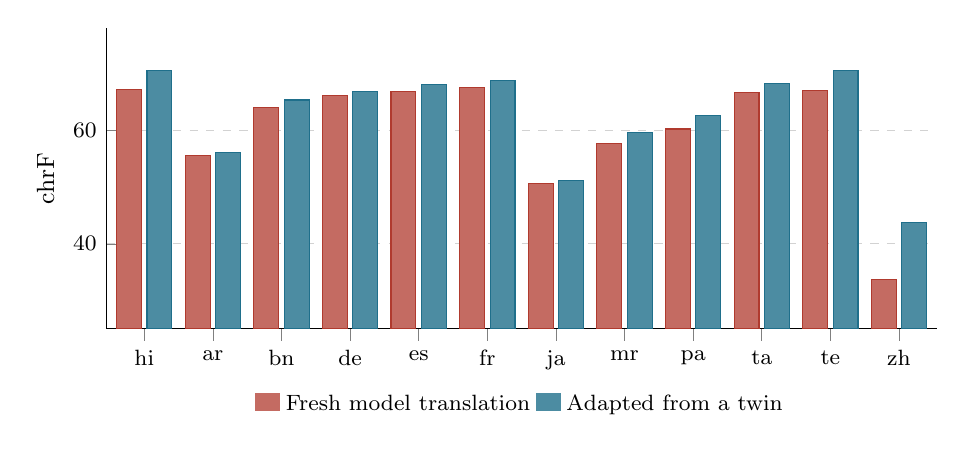
\begin{tikzpicture}
\begin{axis}[reportbars, width=\linewidth, height=5.4cm, bar width=9pt,
  symbolic x coords={hi,ar,bn,de,es,fr,ja,mr,pa,ta,te,zh}, xtick=data,
  ylabel={chrF}, ymin=25, ymax=78, enlarge x limits=0.05]
\addplot[fill=cprev!75, draw=cprev] coordinates {(hi,67.12) (ar,55.51) (bn,64.10) (de,66.12) (es,66.82) (fr,67.54) (ja,50.62) (mr,57.62) (pa,60.24) (ta,66.62) (te,66.98) (zh,33.78)};
\addplot[fill=cnew!80, draw=cnew] coordinates {(hi,70.62) (ar,56.08) (bn,65.34) (de,66.83) (es,68.04) (fr,68.74) (ja,51.14) (mr,59.55) (pa,62.60) (ta,68.28) (te,70.50) (zh,43.82)};
\legend{Fresh model translation, Adapted from a twin}
\end{axis}
\end{tikzpicture}
\caption[Near-twin reuse per language]{Near-twin reuse scores at least as well as fresh translation in every language.}
\label{fig:twins}
\end{figure}

\paragraph{Finding.} By chrF, adapted translations score \textbf{equal or higher in all twelve languages} (mean 62.63
against 60.26), with placeholders kept 100\% in both. chrF rewards consistency: the model translates each string in
isolation and may translate ``Points'' one way in ``42 Points'' and another in ``78 Points'', while reuse applies the same
translation to every twin. A COMET check on the strings where reuse actually changed the output
(Chapter~\ref{sec:tmexp}) shows \textbf{equal} quality rather than higher, so the benefit of reuse is saved model work
and a more consistent application, at unchanged quality. Refusals
(8\%) were mostly strings whose numbers the model wrote in local digits; those strings were simply translated as before.
Near-twin reuse is enabled by default.

\section{Translation Memory Experiment: Simulated CI/CD Commits}
\label{sec:tmexp}

\subsection{Design}
A Translation Memory pays off only \emph{across} runs, when the same application is translated again after a change. The
experiment therefore reproduces a commit history (Table~\ref{tab:versions}): a first release, then commits that add 1\%,
5\% and 10\% new strings. Each commit size was run three times (r1--r3), and every commit's new strings are used in no
other version, so the memory has genuinely never seen them. The new strings are real KDE4 strings held back from the
first release, so they have reference translations.

\begin{table}[H]
\centering
\caption[Application versions]{Application versions used in the experiment (12 languages each).}
\label{tab:versions}
\begin{tabular}{@{}l l S[table-format=5.0]@{}}
\toprule
\textbf{Version} & \textbf{Content} & {\textbf{Translations}} \\
\midrule
v1 & 2,000 random KDE4 strings (first release) & 24000 \\
v2 & v1 + 20 new strings (1\% commit) & 24240 \\
v3 & v1 + 100 new strings (5\% commit) & 25200 \\
v4 & v1 + 200 new strings (10\% commit) & 26400 \\
\bottomrule
\end{tabular}
\end{table}

All steps ran in sequence on one m5.large, keeping the memory between steps as a CI server would (run
\code{ec2-20261017t175415z}). As the comparison point, the final step re-ran v4 with the memory emptied and near-twin
reuse switched off, which is the pipeline as it was before this work. The previous pipeline's time for v2 and v3 was
calculated from that step's measured rate (0.1046~s per translation). This is justified because, with nothing reused, time
grows linearly with the number of translations: the first release, which also reused nothing, ran at 0.1039~s.

A 2,000-string application was used instead of all 10,054 strings to keep the experiment to about two and a half hours
and to allow three repeats. The savings are proportions, so they do not depend on application size, and full-scale speed
is known from Chapter~\ref{sec:kde4run}.

\subsection{Results per Step}
\begin{table}[H]
\centering
\caption[Every step of the memory experiment]{Every step of the experiment. ``Work'' is time spent translating the files;
``Step'' adds about 30~s of fixed start-up per run (image check, model download and load).}
\label{tab:tmsteps}
\small\setlength{\tabcolsep}{4pt}
\begin{tabular}{@{}l S[table-format=5.0] S[table-format=5.0] S[table-format=3.0] S[table-format=5.0] S[table-format=4.1] S[table-format=4.1] S[table-format=6.0]@{}}
\toprule
\textbf{Step} & {\textbf{Translations}} & {\textbf{Memory hits}} & {\textbf{Twins}} & {\textbf{To model}} & {\textbf{Work (s)}} & {\textbf{Step (s)}} & {\textbf{Model tokens}} \\
\midrule
v1 (empty memory) & 24000 & 0 & 365 & 23650 & 2492.7 & 2578.9 & 261431 \\
v2-r1 (+1\%) & 24240 & 23883 & 0 & 357 & 54.6 & 93.4 & 3972 \\
v3-r1 (+5\%) & 25200 & 23883 & 59 & 1261 & 155.5 & 186.9 & 13706 \\
v4-r1 (+10\%) & 26400 & 23883 & 71 & 2446 & 287.5 & 319.4 & 26468 \\
v2-r2 & 24240 & 23883 & 12 & 345 & 55.6 & 86.9 & 4051 \\
v3-r2 & 25200 & 23883 & 33 & 1284 & 168.0 & 199.4 & 13957 \\
v4-r2 & 26400 & 23883 & 81 & 2436 & 316.7 & 348.4 & 27646 \\
v2-r3 & 24240 & 23883 & 0 & 357 & 96.4 & 127.8 & 4816 \\
v3-r3 & 25200 & 23883 & 12 & 1305 & 152.6 & 184.0 & 13664 \\
v4-r3 & 26400 & 23883 & 59 & 2458 & 295.0 & 327.3 & 27746 \\
\midrule
v4, previous pipeline & 26400 & 0 & 0 & 26415 & 2761.1 & 2794.2 & 290622 \\
\bottomrule
\end{tabular}
\end{table}

All 132 language files succeeded. The 117 misses among the unchanged strings in each later step are the Chinese and
Japanese strings kept in English (Chapter~\ref{sec:quality}), which were not yet remembered at this stage
(Chapter~\ref{sec:bottlenecks}).

\subsection{New Pipeline against the Previous Pipeline}
\begin{table}[H]
\centering
\caption[New pipeline against the previous pipeline]{Averages of three repeats against the previous pipeline.
Previous-pipeline values for +1\% and +5\% are calculated from its measured rate; +10\% is measured. Cost uses \$0.101 per
machine-hour.}
\label{tab:tmheadline}
\small\setlength{\tabcolsep}{3.5pt}
\begin{tabular}{@{}l S[table-format=4.0] S[table-format=3.1] S[table-format=2.1] S[table-format=6.0] S[table-format=5.0] S[table-format=2.1] c@{}}
\toprule
\textbf{Commit} & {\textbf{Previous (s)}} & {\textbf{New (s)}} & {\textbf{Speed-up}} & {\textbf{Tokens, prev.}} & {\textbf{Tokens, new}} & {\textbf{Saved (\%)}} & \textbf{Cost per run} \\
\midrule
+1\% & 2568 & 102.7 & 25.0 & 266844 & 4280 & 98.4 & \$0.072 $\rightarrow$ \$0.0029 \\
+5\% & 2669 & 190.1 & 14.0 & 277412 & 13776 & 95.0 & \$0.075 $\rightarrow$ \$0.0053 \\
+10\% & 2794 & 331.7 & 8.4 & 290622 & 27287 & 90.6 & \$0.078 $\rightarrow$ \$0.0093 \\
\bottomrule
\end{tabular}
\end{table}

\begin{figure}[H]
\centering
\begin{subfigure}[t]{0.48\linewidth}
\centering
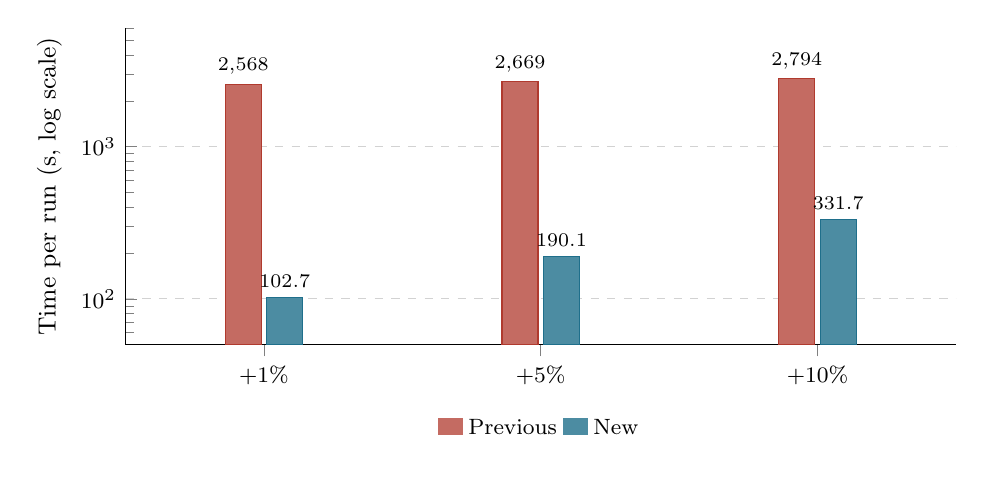
\begin{tikzpicture}
\begin{axis}[reportbars, width=\linewidth, height=5.6cm, bar width=13pt,
  symbolic x coords={+1\%,+5\%,+10\%}, xtick=data, ymode=log, log origin=infty,
  ymin=50, ymax=6000, ylabel={Time per run (s, log scale)},
  nodes near coords, point meta=rawy, nodes near coords style={font=\scriptsize}, enlarge x limits=0.25,
  legend style={at={(0.5,-0.2)}}]
\addplot[fill=cprev!75, draw=cprev] coordinates {(+1\%,2568) (+5\%,2669) (+10\%,2794)};
\addplot[fill=cnew!80, draw=cnew] coordinates {(+1\%,102.7) (+5\%,190.1) (+10\%,331.7)};
\legend{Previous, New}
\end{axis}
\end{tikzpicture}
\caption{Time per run}
\end{subfigure}\hfill
\begin{subfigure}[t]{0.48\linewidth}
\centering
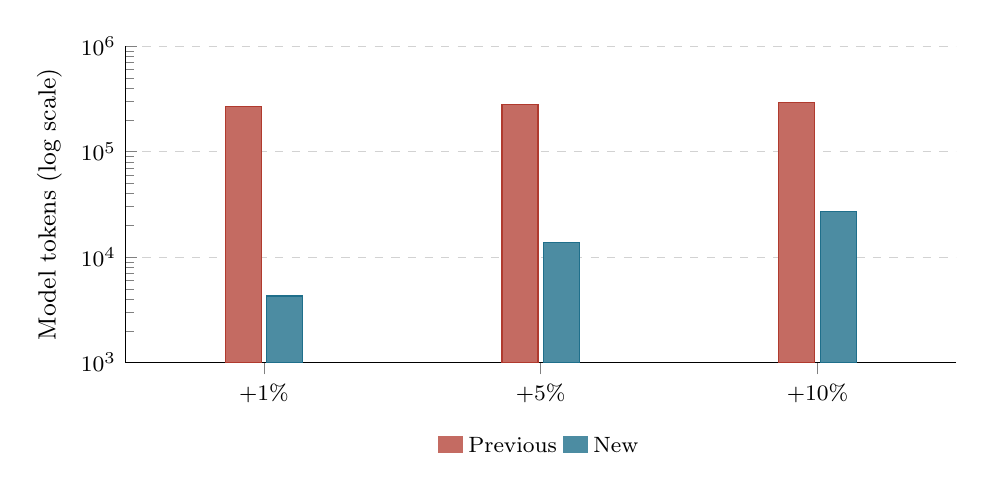
\begin{tikzpicture}
\begin{axis}[reportbars, width=\linewidth, height=5.6cm, bar width=13pt,
  symbolic x coords={+1\%,+5\%,+10\%}, xtick=data, ymode=log, log origin=infty,
  ymin=1000, ymax=1000000, ylabel={Model tokens (log scale)},
  enlarge x limits=0.25, legend style={at={(0.5,-0.2)}}]
\addplot[fill=cprev!75, draw=cprev] coordinates {(+1\%,266844) (+5\%,277412) (+10\%,290622)};
\addplot[fill=cnew!80, draw=cnew] coordinates {(+1\%,4280) (+5\%,13776) (+10\%,27287)};
\legend{Previous, New}
\end{axis}
\end{tikzpicture}
\caption{Model tokens per run}
\end{subfigure}
\caption[Time and model tokens per commit]{The previous pipeline's cost is fixed by application size; the new pipeline's
cost follows the size of the change.}
\label{fig:tmcommits}
\end{figure}

\paragraph{Why smaller commits gain more.} The previous pipeline retranslated everything, so its time was about 45 minutes
whatever changed. The new pipeline's time follows the size of the change, so the ratio is largest for small commits, which
are the common case in CI/CD. A 1\% commit did not reach the ideal 100\x{} for three reasons, each addressed in
Chapter~\ref{sec:bottlenecks}: a fixed start-up of about 30~s per run; the 117 kept-English strings, which were sent to the
model again on every run (a third of a 1\% commit's model work); and small batches, which used the model less efficiently
(58--85\% padding against 16\% when translating everything).

\subsection{Quality, Lookups and Near-Twins}
\begin{table}[H]
\centering
\caption[Quality, lookups and near-twins]{Quality, database lookups and near-twin reuse.}
\label{tab:tmquality}
\begin{tabularx}{\linewidth}{@{}l L@{}}
\toprule
\textbf{Measure} & \textbf{Result} \\
\midrule
Quality, v4 from the memory & chrF \textbf{63.38}, placeholders kept 100\%, 0 missing \\
Quality, v4 previous pipeline & chrF \textbf{63.37}, placeholders kept 100\%, 0 missing \\
Database queries per run & \textbf{12} (one per language) against 36 for the previous per-file, per-1,000-string queries \\
Time to load the memory & 224--272~ms in total for all 12 languages; every later check is in-process \\
Near-twins in the first release & 365 of 24,000 translations (1.5\%) reused instead of translated \\
\bottomrule
\end{tabularx}
\end{table}

Quality is unchanged because a memory hit returns exactly the translation that the same engine produced earlier, which the
engine label guarantees. Near-twins were rarer in the 2,000-string application (1.5\%) than in the full corpus (5.2\%),
because a twin helps only when its partner is also present.

\keyresult{\textbf{RQ5.} Under simulated CI/CD commits, the redesigned memory made 1\%, 5\% and 10\% commits 25\x{},
14\x{} and 8.4\x{} faster than the previous pipeline, with 98.4\%, 95.0\% and 90.6\% fewer model tokens and unchanged
quality (chrF 63.38 against 63.37). Database queries fell from 36 to 12 per run.}

\section{Removing the Remaining Per-Run Costs}
\label{sec:bottlenecks}

\subsection{Where a CI Run Spends Its Time}
The experiment in Chapter~\ref{sec:tmexp} ran on one machine that stayed on between steps. That measures the memory
fairly, but it hides the cost a real CI run pays on \emph{every} commit: starting a machine and preparing it. Timing a
small commit end to end showed four remaining costs (Table~\ref{tab:runcosts}).

\begin{table}[H]
\centering
\caption[Remaining per-run costs]{Per-run costs that remained after the Translation Memory redesign.}
\label{tab:runcosts}
\begin{tabularx}{\linewidth}{@{}l r L@{}}
\toprule
\textbf{Part of one CI run} & \textbf{Time} & \textbf{Cause} \\
\midrule
Start and stop a fresh machine & $\sim$106 s & a new machine boots and installs Docker for every commit \\
Image build and model set-up & $\sim$80 s & the container image is built from scratch; the 629~MB model was copied into the image although it is mounted at run time; the model was downloaded and test-loaded every run \\
Kept-English strings & $\sim$23 s & strings stored as untranslatable were not remembered, so 117 went back to the model on every run with the same result \\
Small model calls & -- & $\sim$30 new strings per language form one batch, so one of the two engine workers is idle \\
\bottomrule
\end{tabularx}
\end{table}

\subsection{Fixes}
\begin{enumerate}
  \item \textbf{Model kept out of the image build.} A build-ignore rule excludes the model folder, which the translator
        mounts at run time.
  \item \textbf{Kept-English strings remembered.} They are saved with an empty translation for the current engine version.
        Later runs skip the model for them and still list them for a translator; a new engine version retries them.
  \item \textbf{Ready runner.} Instead of a fresh machine per commit, one runner is kept \emph{stopped} between runs and
        started when needed. Its disk keeps the built image and the model, so a run skips the build and the download, and a
        model already present for the current version also skips its test load. The runner is stopped, not deleted, after
        each run.
  \item \textbf{Balanced small batches.} A model call small enough for two batches is split into two length-sorted batches
        of equal tokens, one per engine worker. Large calls are unchanged.
\end{enumerate}

\subsection{Measured Before and After}
One 5\% commit was timed end to end, from launch to result, with the code before these fixes on a fresh machine (as CI ran
until then) and with the current code on the ready runner, on the same day and machine type
(runs \code{ec2-20261018t143022z} and \code{ec2-20261018t143618z}).

\begin{table}[H]
\centering
\caption[One 5\% commit before and after the fixes]{One 5\% commit end to end, before and after the fixes. Both runs completed all 12 files with no failures.}
\label{tab:beforeafter}
\begin{tabular}{@{}l S[table-format=3.1] S[table-format=3.1] S[table-format=2.1]@{}}
\toprule
\textbf{Part} & {\textbf{Before (s)}} & {\textbf{After (s)}} & {\textbf{Saved (s)}} \\
\midrule
Start and stop the machine & 106.1 & 37.5 & 68.6 \\
Image and model set-up & 79.5 & 18.7 & 60.8 \\
Translation work & 168.1 & 127.2 & 40.9 \\
Phases 1 and 3 & 2.9 & 2.8 & 0.1 \\
\midrule
\textbf{Whole run} & \bfseries 356.6 & \bfseries 186.2 & \bfseries 170.4 \\
\midrule
Strings sent to the model & {1,284} & {1,188} & \\
Machine cost of the run & {\$0.0100} & {\$0.0052} & \\
\bottomrule
\end{tabular}
\end{table}

\begin{figure}[H]
\centering
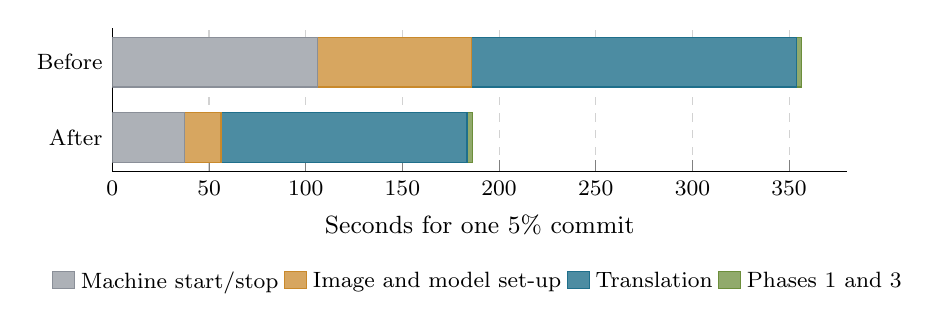
\begin{tikzpicture}
\begin{axis}[xbar stacked, width=0.9\linewidth, height=3.4cm, bar width=18pt, enlarge y limits=0.45,
  axis lines*=left, xmajorgrids, grid style={dashed,gray!35},
  symbolic y coords={After,Before}, ytick=data, xmin=0, xmax=380,
  xlabel={Seconds for one 5\% commit}, tick label style={font=\footnotesize}, label style={font=\small},
  legend style={font=\footnotesize, draw=none, legend columns=4, at={(0.5,-0.62)}, anchor=north}]
\addplot[fill=cgrey!70, draw=cgrey] coordinates {(106.1,Before) (37.5,After)};
\addplot[fill=cfourth!75, draw=cfourth] coordinates {(79.5,Before) (18.7,After)};
\addplot[fill=cnew!80, draw=cnew] coordinates {(168.1,Before) (127.2,After)};
\addplot[fill=cthird!75, draw=cthird] coordinates {(2.9,Before) (2.8,After)};
\legend{Machine start/stop, Image and model set-up, Translation, Phases 1 and 3}
\end{axis}
\end{tikzpicture}
\caption[Composition of one 5\% commit]{Composition of one 5\% commit before and after the fixes: 5.9 minutes to 3.1 minutes (1.9\x{}).}
\label{fig:beforeafter}
\end{figure}

Each commit must contain strings that are new to the memory, so the two runs used different 5\% versions (v3-r2 and
v3-r3); with the previous code, v3-r3 needed about 9\% less translation work than v3-r2. Table~\ref{tab:samecommit}
therefore compares translation work on the \emph{same} commits.

\begin{table}[H]
\centering
\caption[Translation work on the same commits]{Translation work on the same commits with the previous code (Chapter~\ref{sec:tmexp}) and the current code.}
\label{tab:samecommit}
\begin{tabular}{@{}l c S[table-format=3.1] S[table-format=3.1] S[table-format=3.0]@{}}
\toprule
\textbf{Commit} & \textbf{Strings to model} & {\textbf{Before (s)}} & {\textbf{After (s)}} & {\textbf{Change (\%)}} \\
\midrule
+1\% (v2-r1) & 357 $\rightarrow$ 240 & 54.6 & 38.2 & -30 \\
+1\% (v2-r2) & 345 $\rightarrow$ 228 & 55.6 & 39.2 & -29 \\
+1\% (v2-r3) & 357 $\rightarrow$ 240 & 96.4 & 74.5 & -23 \\
+5\% (v3-r1) & 1,261 $\rightarrow$ 1,144 & 155.5 & 127.4 & -18 \\
+5\% (v3-r3) & 1,305 $\rightarrow$ 1,188 & 152.6 & 127.2 & -17 \\
+10\% (v4-r1) & 2,446 $\rightarrow$ 2,329 & 287.5 & 252.1 & -12 \\
\bottomrule
\end{tabular}
\end{table}

\subsection{Contribution of Each Fix}
\begin{itemize}
  \item \textbf{Ready runner and image fix:} machine start and stop fell from about 106~s to 37--44~s, and image and model
        set-up from about 80~s to 19--36~s (four runs on the ready runner). Together this saves about two minutes on every
        CI run, whatever the size of the commit: the largest gain.
  \item \textbf{Remembered kept-English strings:} exactly 117 fewer strings sent to the model per commit; all 117 were
        found in the memory instead. This is most of the saving on small commits.
  \item \textbf{Balanced small batches:} about 8--10\% less time per translated string on 5\% and 10\% commits
        (0.123 to 0.111~s, and 0.118 to 0.108~s), but no measurable gain on 1\% commits, where fixed per-file costs
        outweigh model time.
\end{itemize}

With all fixes, measured end to end on the ready runner, a 1\% commit took 156.9~s, a 5\% commit 186.0--186.2~s and a 10\%
commit 312.2~s. The stopped runner's 40~GB disk costs \$3.65 per month whether it is used or not.

\keyresult{\textbf{RQ6.} Starting a fresh machine, rebuilding the image and re-sending untranslatable strings cost about
three minutes per CI run. Removing them cut a 5\% commit, measured end to end, from 5.9 to 3.1 minutes (1.9\x{}).}

\section{Semester Trajectory}
\label{sec:trajectory}

Figure~\ref{fig:trajectory} follows one 5\% commit (2,100 strings, 25,200 translations) through the semester. Each stage
changes one part of the pipeline.

\begin{figure}[H]
\centering
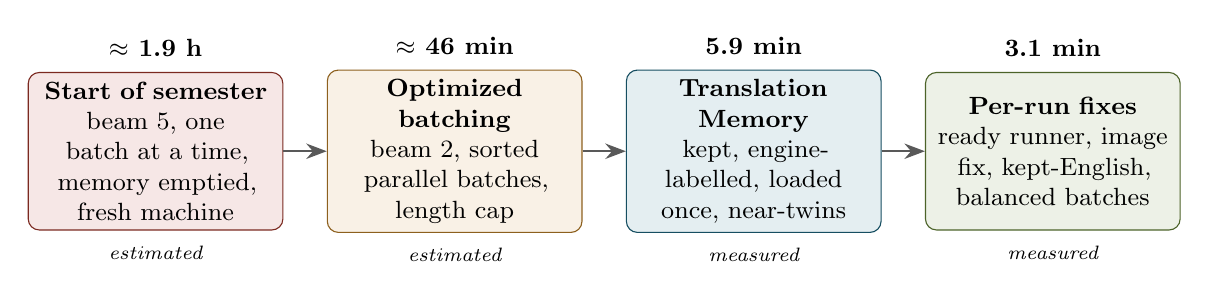
\begin{tikzpicture}[
  stage/.style={draw=#1!70!black, fill=#1!12, rounded corners=4pt, align=center, font=\small, text width=3.0cm, minimum height=2.0cm},
  arr/.style={-{Stealth[length=2.6mm]}, thick, draw=black!65},
  val/.style={font=\bfseries\small, above=2pt},
  sub/.style={font=\scriptsize\itshape, below=2pt, align=center}]
\node[stage=cprev] (s1) {\textbf{Start of semester}\\beam 5, one batch at a time, memory emptied, fresh machine};
\node[stage=cfourth, right=0.55cm of s1] (s2) {\textbf{Optimized batching}\\beam 2, sorted parallel batches, length cap};
\node[stage=cnew, right=0.55cm of s2] (s3) {\textbf{Translation Memory}\\kept, engine-labelled, loaded once, near-twins};
\node[stage=cthird, right=0.55cm of s3] (s4) {\textbf{Per-run fixes}\\ready runner, image fix, kept-English, balanced batches};
\node[val] at (s1.north) {$\approx$ 1.9 h};
\node[val] at (s2.north) {$\approx$ 46 min};
\node[val] at (s3.north) {5.9 min};
\node[val] at (s4.north) {3.1 min};
\node[sub] at (s1.south) {estimated};
\node[sub] at (s2.south) {estimated};
\node[sub] at (s3.south) {measured};
\node[sub] at (s4.south) {measured};
\draw[arr] (s1) -- (s2);
\draw[arr] (s2) -- (s3);
\draw[arr] (s3) -- (s4);
\end{tikzpicture}
\caption[Semester trajectory of one 5\% commit]{One 5\% commit, end to end, across the semester's stages.}
\label{fig:trajectory}
\end{figure}

\begin{table}[H]
\centering
\caption[Sources of the trajectory times]{How each stage's time for a 5\% commit was obtained.}
\label{tab:trajectory}
\begin{tabularx}{\linewidth}{@{}l r L@{}}
\toprule
\textbf{Stage} & \textbf{Time} & \textbf{Source} \\
\midrule
Start of semester & $\approx$1.9 h & 25,200 translations at the benchmark rate of 13,631 per hour (Table~\ref{tab:kde4beam}), plus machine start and set-up \\
Optimized batching & $\approx$46 min & 25,200 translations at the previous pipeline's measured 0.1046~s each (Chapter~\ref{sec:tmexp}), plus machine start \\
Translation Memory & 5.9 min & measured end to end on a fresh machine (Table~\ref{tab:beforeafter}, ``before'') \\
Per-run fixes & 3.1 min & measured end to end on the ready runner (Table~\ref{tab:beforeafter}, ``after'') \\
\bottomrule
\end{tabularx}
\end{table}

Batching made every model call cheaper (about 2.5\x{} at full scale); the Translation Memory removed most model calls
altogether; and the per-run fixes removed most of the set-up around them. Overall, a typical commit went from roughly
1.9 hours to 3.1 minutes, while quality was preserved at every step: identical output for batching layout and parallelism,
a 0.45-point chrF trade-off for beam~2, more placeholders kept, and unchanged chrF with the memory.

\section{Engineering Decisions and Rationale}
\label{sec:decisions}

\subsection{Why beam 2 rather than beam 1?}
Beam~1 is faster (3.46\x{} against 2.20\x{} on KDE4) but loses 2.15 chrF overall and about six points for Chinese and
Japanese. Beam~2 keeps every language within 1.4 points of beam~5 for more than twice the speed.

\subsection{Why not larger batches or cross-file batching?}
Batch layout changed speed by at most 3\% while doubling peak memory, and a 4,096-token attempt did not complete on the
8~GB machine. Batches are therefore kept at 1,024 tokens and per file, which also preserves per-file telemetry.

\subsection{Why square markers for placeholders?}
They survived translation in 99.15\% of cases against 88.78\% and 80.66\% for the alternatives, because the model copies
citation-style markers such as \code{[1]} unchanged.

\subsection{Why keep untranslatable strings in English?}
Forcing the model to avoid \code{<unk>} produced fluent but wrong words. An English string in a localized application is
visible and can be fixed by a translator; a wrong word is silent.

\subsection{Why a hash as the memory key?}
SQL Server limits a key to 900 bytes (434 characters). A fixed 32-byte SHA-256 hash removes the limit while keeping
lookups indexed.

\subsection{Why record the engine version with each translation?}
It makes reuse safe across model and setting changes without manual cleanup: older entries simply stop matching.

\subsection{Why base punctuation rules on counts?}
The first, guessed rules made Japanese reuse worse than fresh translation. Counting how every reference ends turned the
result from a loss into a gain.

\subsection{Why test the memory with commit-like versions?}
A memory only pays off across runs. Versions with genuinely new strings, run in sequence with the memory kept, measure
the savings a CI server would actually see, rather than a seeded cache rate.

\subsection{Why a stopped ready runner?}
A stopped machine keeps its disk (the built image and the model) for \$3.65 per month and starts in seconds, saving about
two minutes per CI run over a fresh machine.

\section{Cost and Reliability}
\label{sec:cost}

\subsection{Cost}
All costs below are machine time at the on-demand price of an m5.large in \code{ap-south-1} (\$0.101 per hour). The
database and storage cost the same regardless of the pipeline version and are not included.

\begin{table}[H]
\centering
\caption[Machine cost per run]{Machine cost per run.}
\label{tab:cost}
\begin{tabularx}{\linewidth}{@{}L r r@{}}
\toprule
\textbf{Run} & \textbf{Machine time} & \textbf{Cost} \\
\midrule
Full KDE4 corpus, 12 languages (120,648 translations) & 3 h 38 min & \$0.367 \\
\quad per 1,000 translations & & \$0.0030 \\
5\% commit, previous pipeline (memory emptied, calculated) & $\approx$46 min & $\approx$\$0.075 \\
5\% commit, new memory, fresh machine (measured) & 5.9 min & \$0.0100 \\
5\% commit, all fixes, ready runner (measured) & 3.1 min & \$0.0052 \\
Ready runner disk while stopped (40 GB gp3) & -- & \$3.65 per month \\
\bottomrule
\end{tabularx}
\end{table}

Per run the amounts are small, but a CI pipeline runs on every commit, often many times a day and for many applications
and languages, so a 93\% saving per commit compounds. The larger benefit is time: developers receive localized resources
in about three minutes instead of most of an hour.

\subsection{Reliability}
Every recorded run in this report completed without translation failures: 12 of 12 files in the full KDE4 run, 24 of 24
in the check run, 132 of 132 in the memory experiment, and 12 of 12 in each end-to-end commit. Phase~2 also treats any
swallowed inference error, missing segments or storage error as a failed file instead of a silent success, isolates
failures per file so that one bad file does not stop the others, and keeps unprocessed files in S3 for a retry. The
code is covered by an automated test suite of 254 tests.

\section{Limitations and Future Work}
\label{sec:limitations}

\subsection{Limitations}
\begin{itemize}
  \item \textbf{Reference translations.} The KDE4 references appear to be machine-generated (Chapter~\ref{sec:setup}), so
        chrF measures closeness to them rather than to human translation. Comparisons between pipeline versions are
        unaffected because all versions use the same references.
  \item \textbf{Calculated baselines.} The previous pipeline's times for 1\% and 5\% commits, and the start-of-semester
        stage in Chapter~\ref{sec:trajectory}, are calculated from measured rates; each is labelled.
  \item \textbf{One machine type and short strings.} All timings are for an m5.large and for user-interface strings with
        a median length of two words. Longer text would change absolute times, not the conclusions about what dominates them.
  \item \textbf{Experiment size.} The memory experiment used a 2,000-string application, in which near-twins are rarer
        than in the full corpus (1.5\% against 5.2\%).
  \item \textbf{Metric coverage.} This report uses chrF and placeholder survival; BLEU, ROUGE-L, METEOR and COMET are
        computed by Track~1.
\end{itemize}

\subsection{Future Work}
\begin{itemize}
  \item Repeat the memory experiment at full scale (10,054 strings) to confirm the savings on a production-size application.
  \item Compare machine types, including newer CPUs and GPUs, by cost per 1,000 translations.
  \item Evaluate beam~1 for the languages where its loss was smallest (under 1.3 chrF for Hindi, Marathi, Punjabi and
        Bengali), keeping beam~2 for Chinese and Japanese.
  \item Store the memory as per-language files in S3 now that it is loaded once per run, removing the always-on database.
\end{itemize}

\section{Conclusion}
\label{sec:conclusion}

This semester moved the localization pipeline to AWS and reduced the work it does on every commit. Profiling showed that
model inference takes 99.3\% of the translation stage. A one-change-at-a-time study then showed that the common intuition
about batching, that less padding means more speed, does not hold here: padding fell from 30\% to 4\% for a 3\% gain,
while the beam size and idle cores were the real costs. With beam~2, parallel batches and an output length cap, the
production pipeline translated the full twelve-language KDE4 corpus, 120,648 translations, in 3.6 hours with no failures,
about 2.5\x{} faster than at the start of the semester.

Scale exposed problems that small tests could not: broken placeholders and characters the model cannot write. Placeholder
protection raised survival from 87.7\% to 99.88\%, and untranslatable strings are now kept in English and reported rather
than shipped broken.

The redesigned Translation Memory changed the economics of the pipeline. Because it persists, records the engine that
produced each entry, loads once per language and reuses near-identical strings, the cost of a run now follows the size of
the change rather than the size of the application: 1\%, 5\% and 10\% commits ran 25\x{}, 14\x{} and 8.4\x{} faster with
90--98\% fewer model tokens and unchanged quality. Removing the remaining per-run set-up brought a typical 5\% commit to
3.1 minutes end to end, from roughly 1.9 hours at the start of the semester.


\clearpage
\begin{thebibliography}{9}
\addcontentsline{toc}{section}{References}

\bibitem{nllb}
NLLB Team, M.~R. Costa-juss\`a, J.~Cross, et al.
\newblock No Language Left Behind: Scaling Human-Centered Machine Translation.
\newblock \emph{arXiv:2207.04672}, 2022.

\bibitem{ct2}
OpenNMT.
\newblock CTranslate2: Fast inference engine for Transformer models.
\newblock \url{https://github.com/OpenNMT/CTranslate2}.

\bibitem{opus}
J.~Tiedemann.
\newblock Parallel Data, Tools and Interfaces in OPUS.
\newblock In \emph{Proceedings of LREC}, 2012.

\bibitem{chrf}
M.~Popovi\'c.
\newblock chrF: character n-gram F-score for automatic MT evaluation.
\newblock In \emph{Proceedings of the Tenth Workshop on Statistical Machine Translation}, 2015.

\bibitem{sacrebleu}
M.~Post.
\newblock A Call for Clarity in Reporting BLEU Scores.
\newblock In \emph{Proceedings of the Third Conference on Machine Translation}, 2018.

\bibitem{comet}
R.~Rei, J.~G.~C. de~Souza, D.~Alves, et al.
\newblock COMET-22: Unbabel-IST 2022 Submission for the Metrics Shared Task.
\newblock In \emph{Proceedings of the Seventh Conference on Machine Translation}, 2022.

\bibitem{flores}
N.~Goyal, C.~Gao, V.~Chaudhary, et al.
\newblock The FLORES-101 Evaluation Benchmark for Low-Resource and Multilingual Machine Translation.
\newblock \emph{Transactions of the Association for Computational Linguistics}, 10, 2022.

\end{thebibliography}

\appendix
\section{Telemetry Fields Added This Semester}
\label{app:telemetry}
Each translated file emits one \code{RESEARCH\_DATA} record. The previous semester's fields are unchanged; Table~\ref{tab:newfields}
lists the fields added this semester.

\begin{table}[H]
\centering
\caption[New telemetry fields]{New \code{RESEARCH\_DATA} fields.}
\label{tab:newfields}
\begin{tabularx}{\linewidth}{@{}l L@{}}
\toprule
\textbf{Field} & \textbf{Meaning} \\
\midrule
\code{cloud\_provider}, \code{region}, \code{run\_id} & where and in which run the file was translated \\
\code{cpu\_limit}, \code{cpu\_model}, \code{host\_cpu\_count} & cores available to the translator and the host CPU \\
\code{tm\_db\_queries} & database queries made for this file (0 after the language is loaded) \\
\code{tm\_lookup\_ms} & time spent on memory lookups \\
\code{tm\_hits\_in\_run} & hits on entries translated earlier in the same run \\
\code{tm\_twin\_hits} & strings adapted from a near-twin \\
\code{tm\_kept\_english} & strings remembered as kept in English \\
\code{model\_strings} & strings sent to the model, including placeholder fallbacks \\
\code{real\_input\_tokens}, \code{real\_output\_tokens} & tokens read and written by the model (tokenizer counts) \\
\code{padding\_pct} & share of padded input positions in this file's batches \\
\bottomrule
\end{tabularx}
\end{table}

\section{Recorded Runs}
\label{app:runs}
All runs used an m5.large in \code{ap-south-1}. Outputs are stored in S3 under \code{runs/<run-id>/}, and logs and telemetry
in CloudWatch Logs.

\begin{table}[H]
\centering
\caption[Recorded runs]{Runs referenced in this report.}
\label{tab:runs}
\begin{tabularx}{\linewidth}{@{}l L l@{}}
\toprule
\textbf{Run} & \textbf{Content} & \textbf{Chapter} \\
\midrule
\code{ec2-20261015t233954z} & first AWS run, 50 strings $\times$ 7 languages & \ref{sec:arch} \\
\code{ec2-20261016t103748z} & batch layout and beam size, \code{.resx} workload and FLORES-200 & \ref{sec:batching} \\
\code{ec2-20261016t115802z} & beam size on 1,000 KDE4 strings $\times$ 12 languages & \ref{sec:batching} \\
\code{ec2-20261016t142418z} & parallel batches and output length cap & \ref{sec:batching} \\
\code{ec2-20261016t195057z} & placeholder marker styles & \ref{sec:placeholders} \\
\code{ec2-20261016t214343z} & full KDE4 production run & \ref{sec:kde4run} \\
\code{ec2-20261017t063722z} & check run: long strings, \code{<unk>}, memory hits & \ref{sec:quality} \\
\code{ec2-20261017t175415z} & Translation Memory experiment (11 steps) & \ref{sec:tmexp} \\
\code{ec2-20261018t132556z} -- \code{t142626z} & commits with the per-run fixes & \ref{sec:bottlenecks} \\
\code{ec2-20261018t143022z}, \code{t143618z} & 5\% commit before and after the fixes & \ref{sec:bottlenecks} \\
\bottomrule
\end{tabularx}
\end{table}


\end{document}
